\section{Results and Discussion}
\label{sec:result_and_discussion}

%----------------------------------------------------%
% --------- Analysis by Model -----------------------%
%----------------------------------------------------%

\subsection{Analysis by Model}
\label{sec:analysis_by_model}
To give an overview of the field, we present the most predominantly used probabilistic models, give a description, depict their use, and provide an overview of how they are used to create uncertainty estimates for financial time series. Table \ref{table:model_categorization} provides an overview of probabilistic model categories created based on grouping the most commonly used model types. Figure \ref{fig:model_breakdown} illustrates the occurrence of each probabilistic model category, and if they are used independently or in combination with other machine learning or econometric models. The figure shows that while many researchers combine different ML models, few researchers combine ML models with traditional models, indicating a potential gap in the literature. Results and conclusions by model type are summarized in Table \ref{table:conclusions_by_model}.

\begin{table}[H]
    \centering
    \caption[Model Categorization]{Probabilistic Model Categorization.}
    \label{table:model_categorization}
    \small
    \begin{adjustbox}{width=0.5\textwidth,center}
    \begin{tabular}{p{0.2\textwidth}p{0.30\textwidth}}
        \toprule
        \textbf{Model Category} & \textbf{Models} \\
        \midrule
        Bayesian Neural Networks (BNN) & BNN, Gen-BNN, B-TABL \\
        \addlinespace
        \hdashline[0.2pt/3pt]
        \addlinespace
        Gaussian Processes Regression (GPR) & GP, GPR, G4P, GPMCH \\
        \addlinespace
        \hdashline[0.2pt/3pt]
        \addlinespace
        Variational Autoencoders (VAE) & VAE \\
        \addlinespace
        \hdashline[0.2pt/3pt]
        \addlinespace
        Hidden Markov Models (HMM) & HMM, CHMM, MCHMM \\
        \addlinespace
        \hdashline[0.2pt/3pt]
        \addlinespace
        Probabilistic Recurrent Neural Network (P-RNN) Extensions & DeepAR, DeepARA, P-GRU, QRBiLSTM, ESVM, Bayesian LSTM, Bayes ES-RNN, Clockwork RNN \\
        \addlinespace
        \hdashline[0.2pt/3pt]
        \addlinespace
        Probabilistic Generative Adversial Networks (P-GAN) & cGAN, PredACGAN \\
        \addlinespace
        \hdashline[0.2pt/3pt]
        \addlinespace
        Probabilistic Neural Networks (PNN) & PNN\\
        \addlinespace
        \hdashline[0.2pt/3pt]
        \addlinespace
        Other Bayesian Methods & B-SVR, BGLM, Bayesian Network, MCMC \\
        \addlinespace
        \hdashline[0.2pt/3pt]
        \addlinespace
        Other Probabilistic AI Methods & RSMAN, Recurrent Dictionary Learning (RDL), TV-Entropy, Probabilistic Fuzzy Logic (PFL), Leave-One-Out Cross-Conformal Predictive System (LOO-CCPS), P-SVM, B-HANN, Probabilistic Graphical Model (PGM), Augmented DCNN  \\
        \addlinespace
        \addlinespace
        \bottomrule
    \end{tabular}
    \end{adjustbox}
\end{table}

\begin{figure}[H]
    \centering    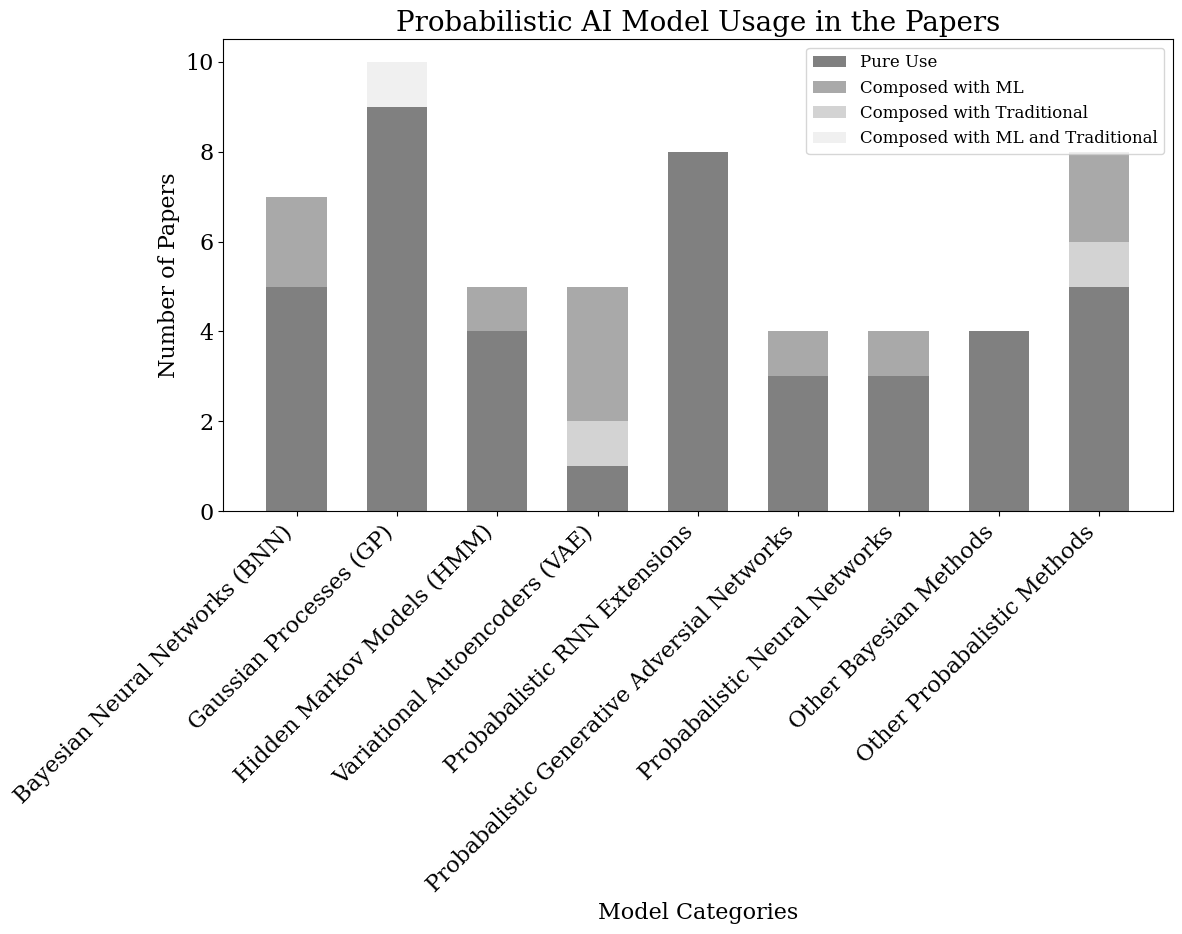
\includegraphics[width=1\linewidth]{Images/model_breakdown.png}
    \caption[Breakdown of probabilistic model categories and usage in papers]{Breakdown of probabilistic model usage in research papers across standalone and hybrid approaches.}
    \label{fig:model_breakdown}
\end{figure}

%--------------------- BNN --------------------------%

\subsubsection{Bayesian Neural Networks (BNNs)}
\label{sec:bnn}

A Bayesian Neural Network (BNN) extends a traditional neural network by integrating Bayesian inference principles, allowing for the modeling of uncertainty in the network parameters \parencite{neal1995bayesian}. Conventional neural networks for time series define a mapping from inputs $x_t$ to outputs $y_t$, which may be dependent on previous inputs and outputs, using a set of trainable weights and biases $w$, represented by
\begin{equation}
    \begin{gathered}
        y_t = f(x_t, x_{t-1}, ..., x_{t-i},  y_{t-1}, ..., y_{t-i};w),
    \end{gathered}
\end{equation}
where $f$ is the composition of linear transformations and non-linear activation functions across multiple layers. BNNs extend this by providing a probabilistic implementation of a standard neural network where the weights and biases are represented as random variables with probability distributions \parencite{chandra2023bayesian}, allowing the model to capture parameter uncertainty. 

Initially each weight is assigned a prior distribution
\begin{equation}
    \begin{gathered}
        p(w) = \Pi_{i} p(w_i),
    \end{gathered}
\end{equation}
where $p(w)$ represents the joint prior distribution over all weights. Combined with the likelihood of observed data $\mathcal{D} = \{(x_n,y_n)\}_{n=1}^N$ given the weights
\begin{equation}
    \begin{gathered}    
        p(\mathcal{D}|w) = \prod_{n=1}^Np(y_n|x_{1:n}, y_{1:n-1},w),
    \end{gathered}
\end{equation}
we can create the posterior distribution over the weights using Bayes rule \parencite[p. 46]{pml1Book}
\begin{equation}
    \begin{gathered}
        p(w|\mathcal{D}) = \frac{p(\mathcal{D}|w)p(w)}{p(\mathcal{D})}.
    \end{gathered}
    \label{eq:bayes_theorem} 
\end{equation}
Predictions for new inputs $x^*$ are consequently made by integrating over the posterior distribution of the weights
\begin{equation}
    \begin{gathered}
        p(y^*|x^*, x_{1:n}, y_{1:n},\mathcal{D}) = \int p(y^*|x^*,x_{1:n}, y_{1:n},w)p(w|\mathcal{D})dw.
    \end{gathered}
\end{equation}
Modeling a posterior distribution over the weights allows uncertainty in parameters to be captured by the distribution variance, enabling predictive distributions rather than single point predictions. Thus the approach enables probabilistic forecasts, making BNNs particularly suitable for uncertainty quantification \parencite{jospin2022hands}. Due to intractability of the exact posterior \parencite{hernandez2015probabilistic}, approximation methods like Monte Carlo dropout and variational inference are commonly employed. 

Both \textcite{cocco2021predictions} and \textcite{jang2018empirical} employ BNNs for cryptocurrency price predictions, primarily focusing on point prediction accuracy. \textcite{cocco2021predictions} apply a BNN with Monte Carlo approximation to predict daily Bitcoin and Ethereum prices, benchmarking against LSTM and Feed Forward Neural Networks (FFNNs). The BNN underperforms on Bitcoin in terms of MAPE but yield better results for Ethereum, while deployed two-stage models with a Support Vector Regression (SVR) and LSTM or FFNN outperform in all cases. Although the authors use the BNN's outputted quantiles as prediction confidence, the authors are focused on point predictions and do not assess uncertainty. Similarly, \textcite{jang2018empirical} employ a BNN to make point predictions for Bitcoin price and volatility, using blockchain-specific data, outperforming linear regression and SVR on MAPE and RSME. The authors present confidence intervals for price and volatility, which could be used to assess total uncertainty. However, the probabilistic output is not leveraged to integrate these measures, nor is uncertainty explicitly evaluated as focus lie on point prediction accuracy. Notably, predictions frequently exceed the stated upper and lower bounds. 

\textcite{chandra2021bayesian} apply a BNN with Markov Chain Monte Carlo (MCMC) for multi-step stock price forecasting, benchmarking against FFNNs trained with ADAM and SGD. The BNN provide superior point estimates in terms of RSME for all stocks. The authors use the probabilistic output of the BNN to create prediction intervals as a measure of uncertainty. However, the quality or robustness of the estimate is not assessed, and evidently the actual stock price frequently fall outside the bounds for some stocks, indicating an unreliable uncertainty estimate. The authors compare uncertainty levels during and after Covid, showing higher predicted uncertainty during the pandemic.

\textcite{soleymani2022longterm} propose a hybrid model, QuantumPath, combining a BNN with a temporal GAN to predict long-term prices for several S\&P 500 stocks. The BNN predicts the drift and volatility parameters for a Feynman-Dirac integral, which simulate stock trajectories by Monte Carlo, while the temporal GAN generates trajectories by condsidering the most probable paths. The probabilistic BNN output is used to estimate the underlying probability distribution of the stock trajectories, and is therefore used implicitly as a volatility estimate. The models weighted expected values for 30-day predictions outperform ARIMA and Ornstein-Uhlbeck. Even though the trajectories represent a distribution of prices, the uncertainty is not assessed.

\textcite{hortua2024forecasting} employ a Bayesian Neural Network (BNN) to forecast the VIX using a hybrid architecture that integrates WaveNet, a Temporal Convolutional Network (TCN), with Bayesian inference techniques such as the Reparametrization Trick (RT), Flipout, and Multiplicative Normalizing Flows (MNF). The authors apply quantile recalibration to correct the miscalibration tendency in neural networks, addressing potentially unreliable uncertainty estimates due to error overestimation, by aligning observed and expected data proportions within prediction intervals, assessed using Root Mean Squared Calibration Error (RMSCE). The models using MNF demonstrate the most calibrated predictions, and generally superior short-term point predictions compared to ARIMA. 

\textcite{magris2023bayesian} introduce a Bayesian Temporal Augmented Bilinear Neural Network (B-TABL) for forecasting and classifying mid-price changes in Limit Order Books (LOB). Employing a Variational Online Gauss Newton (VOGN) method for Bayesian inference, the model yields better calibrated class probabilities than approaches like Monte Carlo Dropout. Expected Calibration Error (ECE) and Expected Calibration Distance (ECD) are used to evaluate how well predicted probabilities align with actual observed frequencies, assessing model reliability in uncertainty estimation. The BNN framework provides predictive distributions for class probabilities, offering an uncertainty measure the authors interpret as confidence. While VOGN optimizer for B-TABL does not clearly outperform ADAM on standard classification metrics, the authors argue that the model deliver more meaningful classifications due to superior calibration scores. 

Lastly, \textcite{jang2018generative} use a Generative BNN to predict American put option prices of differing moneyness on the S\&P 500 by incorporating prior data from financial models. By extending a standard BNN with domain-specific priors and self-evolving capabilities, the model accounts for data-scarce regions like deep in-the-money or out-of-the-money options. The authors solely focus on point predictions of the price and do not quantify uncertainty in predictions. Compared to standard BNN implementations, a GPR model, and a GARCH implementation, their model is superior in terms of MAPE and RMSE.
%--------------------- GPR ------------%

\subsubsection{Gaussian Process Regression (GPR)}
Gaussian Process Regression (GPR) is a probabilistic AI model that makes no specific assumptions about the functional form of the underlying data, making it well-suited for complex regression tasks. GPR is used to perform inference over functions, defining a distribution over possible functions $f(x)$ that fit the given data \parencite{rasmussen_williams_2006}. Formally, a Gaussian Process (GP)  is defined as: 
\begin{equation}
f(x) \sim \mathcal{GP}(m(x), k(x, x'))
\end{equation}
where $m(x)$ is the mean function $\mathbb{E}(f)$, and $k(x, x')$ is the covariance function, also known as the kernel, defining how function values at point $x$ and $ x'$ effect each other:
\begin{equation}
k(x, x')=Cov(f(x),f(x'))
\end{equation}
Based on the posterior distribution, Bayesian inference (\ref{eq:bayes_theorem}) is applied to determine the most likely function $f$ that fits the data, making it possible to make new predictions as new data is observed \parencite{rasmussen_williams_2006}. GPR provides both a predictive mean \( \mathbb{E}(f_*) \) and a predictive variance \( \mathrm{Var}(f_*) \) given by:

\begin{equation}
\mathrm{Var}(f(x_*)) = k(x_*, x_*)—\mathbf{k}_*^\top (\mathbf{K} + \sigma_n^2 \mathbf{I})^{-1} \mathbf{k}_*
\end{equation}

where \( k(x_*, x_*) \) is the prior variance of the function at the test point \( x_* \), \( \mathbf{k}_* \) is the vector of covariances between \( x_* \) and the training inputs \( \mathbf{X} \), \( \mathbf{K} \) is the covariance matrix of the training inputs, \( \sigma_n^2 \) is the noise variance, and \( \mathbf{I} \) is the identity matrix. This variance quantifies the uncertainty in the prediction at \( x_* \), with contributions from both the prior uncertainty and the information gained from the training data. In this equation, we can consider the term $\sigma_n^2$ to be the aleatoric variance, i.e. the irreducible part of the variance stemming from data uncertainty, while the rest represents epistemic variance. A significant drawback of GPR from a financial perspective is that the aleatoric noise is assumed to be constant, ignoring the heteroscedasticity of financial data. This limitation can be remedied by extending the model to account for heteroscedasticity, which in the sample, only \textcite{Risk2018gpr, tegner2021probabilistic, Platanios2014gpr} do.

There are 14 applications of GPR in the sample, mainly used independently, with only three papers combining it with other ML or traditional models. 

\textcite{Suphawan2022gpr} employ GPR to forecast the Stock Exchange of Thailand (SET). The model is compared to ANN and RNN and demonstrate superior prediction accuracy on traditional error metrics (RMSE, MAE, MAPE, NSE). The authors note that the distributional output makes the GPR model advantageous compared to ANN and RNN models because it allows for prediction results with quantification of uncertainty, but the quality of this uncertainty is not assessed. 

\textcite{Wang2021gpr} incorporate GPR in a multi-scale nonlinear ensemble model to predict price with uncertainty for the S\&P 500, Dow Jones and NASDAQ. The ensemble model use Variational Mode Decomposition (VDM) and an Autoencoder (AE) for feature extraction, and a two-step deep learning setup with RNN and LSTM. The GPR is used in final stage to create interval predictions and uncertainty estimates. The model is benchmarked against a regular GPR, ANN, RNN and LSTM implementations, displaying superiority in MAPE, MSE, RMSE, MAE and SSE for point predictions. Additionally, the interval predictions are assessed on coverage probability metrics like Mean Width Percentage (MWP), Mean Coverage (MC) and Prediction Interval Coverage Probability (PICP), outperforming a standalone GPR. The same authors \parencite{Wang2021gprensemble} present an alternative ensemble (SSA-EWSVM-RNN-GPR) for stock index forecasting. Singular Spectrum Analysis (SSA) is used to decompose the original stock index signal to several components for preprocessing and feature extraction, and Enhanced Weighted Support Vector Machine (EWSVM) forecast the decomposed components, which are then combined with a RNN to make point forecasts. Finally, point predictions are fed into a GPR to generate interval forecasts. MWP and CP are used to validate the interval forecast, scoring better than eight GPR benchmark models. Improved point prediction accuracy is also reported.

\textcite{Li2024gpr} integrate GPR with a graph-aware portfolio selection model with Generalized Gaussian Distribution (GGD) likelihood. The model captures both mean return and variance, used for portfolio selection, but do not account for heteroskedacity in the modeling. The GPR-model's selected portfolios return is compared to traditional methods like UCRP, PAMR and OLMAR, yielding better performance in terms of annualized return, Sharpe ratio, annualized volatility and max drawdown on stock data from NYSE, S\&P and TSE.

\textcite{Platanios2014gpr} propose a Gaussian Process Mixture Conditional Heteroscedasticity (GPMCH) model to forecast price and volatility for currency exchange rates and global large-cap equity indices. The model captures volatility clustering and handle the non-linear dependency, presenting a viable alterative to traditional GARCH models. The authors applies a Pitman-Yor process to better capture skewed and tail heavy data distributions, showing that their their GPMCH outperformed GARCH in volatility predictions.

\textcite{tegner2021probabilistic} use a GPR to transform market option price data into a smooth implied volatility surface, capturing implied volatility across options of various strike prices and maturities. Then values of this surface is forecasted using GPR, enabling predictions of implied volatility and, consequently, future option prices. The results indicate a promising ability to forecast the VIX one week ahead, outperforming a naive forecasting approach, but no other benchmark models are considered.

\textcite{Risk2018gpr} use a GPR to construct portfolio tail risk measures in VaR and TVaR. Monte Carlo simulation is used to generate training data for the GPR model and to evaluate portfolio losses under diverse economic scenarios. The GPR model employs non-parametric spatial modeling, meaning it does not assume a fixed functional form for the relationship between economic scenarios and portfolio losses. Instead, it adapts dynamically based on the data, leveraging the principle that similar economic conditions tend to produce similar portfolio outcomes. This approach reduces bias and variance in risk estimates compared to nested simulations. In one of the advanced models presented, they use heteroskedastic GP (hetGP), which handles scenarios of varying levels of noise more effectively, further enhancing the uncertainty estimates. 

Similarly, \textcite{Min2023BlackLitterman} use a GPR to predict return distributions of several American technology stocks, used to derive investor confidence levels based on prediction standard deviations, integrated in a Black-Litterman framework for portfolio construction. The method is benchmarked against an equal weighting and a Global Minimum Variance (GMV) method, and is not able to clearly outperform the GMV in Sharpe ratio or maximum drawdown. 

The last studies in the sample utilizing GPR—\textcite{Papaioannou2022gpr, Zmuk2020gpr, Park2014gpr, Hendawy2023} and \textcite{DeSpiegeleer2018gpr}—apply GPR for price or return prediction in financial time series and \textcite{Hocht2024gpr} predict forward-looking implied volatility (IVOL), generally demonstrating competitive performance against benchmarked models. However, these works focus primarily on point predictions without assessing the probabilistic outputs of the GPR model or quantifying prediction uncertainty.




%--------------------- VAE --------------------------%


\subsubsection{Variational Autoencoders (VAEs)}
Variational Autoencoders (VAEs) are generative models that combine principles from deep learning and variational inference to learn probabilistic representations of data. Introduced by \textcite{kingma2013auto} as Auto-Encoding Variational Bayes, the model architecture differs from traditional autoencoders by modeling the encoded “latent” space as a random vector instead of a deterministic one.
Similar to a conventional autoencoder, the encoder maps input vector data $x$ to a latent space $z$. However, in contrast to a conventional autoencoder, $z$ does not consist of scalars but instead represents the parameters (mean and variance) of a probability distribution $q_\phi(z|x)$ over the latent variables, where $\phi$ denotes the parameters of the encoder network. The decoder reconstructs the original input data from this latent representation by decoding samples $z \sim q_\phi(z|x)$ through $p_\theta(x|z)$, aiming to model the true distribution
\begin{equation}
    \begin{gathered}
        p_\theta(x) = \int p_\theta(x|z)p(z)dz,
    \end{gathered}
\end{equation}
where the decoder is parameterized by $\theta$. However, since the computation of the exact posterior $p_{\theta}(z|x) = \frac{p_{\theta}(x|z) p_{\theta}(z)}{p_{\theta}(x)}$ is intractable, variational inference over the latent variables is employed to approximate it with $q_\phi(z|x)$ \parencite{kingma2013auto}. As the encoder outputs a distribution over the latent variables, uncertainty can be captured in the latent representation by drawing multiple samples. These samples can then be propagated through the decoder, ultimately resulting in a distribution of reconstructed outputs.


Only one paper apply a VAE independently. \textcite{arian2022encoded} propose Encoded VaR, directly applying VAE to estimate VaR by generating synthetic market scenarios from historical cross-sectional stock returns of the S\&P 500, LSE and FSE. The VAE learns the latent structure of the financial return distributions without relying on parametric assumptions or predefined joint distributions, and in turn generate samples of synthetic returns to be interpreted as potential future outcomes. The VAE architecture allows generation of arbitrarily many samples, enabling reconstruction of a theoretical underlying distribution for VaR calculation. The authors claim to enhance the signal-to-noise ratio present in financial data, and benchmark the VaR estimate against GARCH models. While the model shows competitive results for specific loss functions like Lopez' method \parencite{lopez1998methods}, it does not pass all adequacy tests and is not valid, in contrast to GARCH extensions CaViaR-GARCH and EVT-GARCH. 

Of the papers utilizing VAEs in combination with other models, several use it as a probabilistic input to another model and do not directly infer uncertainty estimates from the probabilistic output of the VAE.  
\textcite{caprioli2023quantifying} apply a VAE for risk management to assess credit portfolio sensitivity to asset correlations. The VAE is used to generate synthetic correlation matrices, simulating various market conditions, used as input in a multi-factor Vasciek model with Monte Carlo simulation to examine how shifts in correlations affect VaR. \textcite{choudhury2020enhancing} use VAEs as a pre-processing tool to denoise NASDAQ stock financial time series before using a stacked LSTM autoencoder to make point predictions. The authors report superior results in point predictions compared to other machine learning models like, but do not assess uncertainty in their forecasts. \textcite{tang2024period} also deploy VAEs for denoising financial time series data by extracting latent representations. The model is combined with a transformer (LPAST), and is used for long-term multi-step point predictions of different financial times series. The proposed method outperforms benchmarked machine learning models in point predictions, but the probabilistic outputs of the VAE are not directly utilized for uncertainty quantification. \textcite{li2020multivariate} combine a multimodal VAE with a LSTM architecture to predict agriculture commodity futures. The VAE is used to extract high-level features and reduce noise for input data in the LSTM, and probabilistic output is not used specifically in predictions. Their proposed model outperforms ARIMA, and machine learning benchmarks like CNNs in point prediction accuracy. 

\textcite{xing2019sentiment} propose an innovative approach by combining VAEs with a RNN to forecast stock volatility. Their model, Sentiment-Aware Volatility Forecasting (SAVING), integrates social media sentiment data to jointly model stock price movements and the sentiment that influences them. This interaction is captured through the VAE's latent variables, from which marginal joint probabilities are inferred. Benchmarked against econometric models GARCH, EGARCH and TARCH, the SAVING model outperforms in terms of negative log-likelihood (NLL).

%--------------------- HMMs --------------------------%

\subsubsection{Hidden Markov Models (HMMs)}
Hidden Markov Models (HMMs) are probabilistic models used to analyze sequential data with underlying unobservable structures, extending Markov chain theory \parencite{Rabiner1989hmm}. In finance, HMMs can be applied to model time series where market states, such as bull or bear markets, periods of low or high volatility, or other economic regimes, are not directly observable. 

The classic HMM consists of a finite set of hidden states $S = \{s_1, s_2, ... s_N\}$ and a corresponding sequence of observable outputs $O = \{o_1, o_2, ... o_T\}$. The model is defined by an initial probability distribution $\pi_i = P(q_1 = s_i)$, state transition probabilities $a_{ij} = P(q_{t+1} = s_j|q_t = s_i)$ and the emission probabilities specifying the likelihood of observations given system state $b_j(o_t) = P(o_t|q_t=s_j)$ \parencite{Rabiner1989hmm}. Consequently, HMMs are capable of producing distributional forecasts by utilizing the predictive probability distribution of future observations
\begin{equation}
        P(o_{T+1}|O) = \sum_{i=1}^{N}P(o_{T+1}|q_{T+1} = s_i)P(q_{T+1} = s_i | O).
\end{equation}
The probabilistic modeling of both hidden states and observations enables the computation of confidence intervals and prediction reliability, facilitating uncertainty estimation of predictions.

Two articles use HMMs to address multi-asset dependencies in financial time series forecasting. \textcite{li2010stochastic} propose a stochastic HMM for forecasting fuzzy time series data, modeling the Taiwan Weighted Stock Index as the hidden states and the New Taiwan dollar against the U.S. dollar as the observable state. While the model performs better compared to a standard HMM implementation in forecasting accuracy, it is not evaluated against any other models. Additionally, focus lie solely on point predictions, without assessing the probabilistic output of the model. \textcite{cao2019multi} extend the multi-factor dependency approach by developing a Multi-Layer Coupled HMM (MCHMM). Unlike \textcite{li2010stochastic} who address dependencies within a single market, \textcite{cao2019multi} capture interactions both within and between markets, specifically between stock and currency markets across different countries. The model is reportedly more accurate than ARIMA and logistic regression in trend prediction of German and Dutch stock markets. However, similar to \textcite{li2010stochastic}, uncertainty in predictions derivable from the probabilistic model output is not assessed.

In \textcite{park2011trend}, historical segments of financial time series are labeled as either up-trending or down-trending using the Perceptually Important Points (PIP) algorithm. Continuous Hidden Markov Models (CHMMs) are subsequently trained to classify out-of-sample data. The results demonstrate that the HMM model significantly outperform Support Vector Machines (SVMs) across most tested assets, including currencies, stock indices, and individual stocks.

\textcite{sher2023exploiting} also forecast categorical return trends, applying HMM alongside several other models to forecast movements in individual technology stocks. Although the details around their specific model implementation are limited, the authors report superior performance from the HMM compared to ARIMA, LSTM and several booster models. The probabilistic output of HMM is leveraged to assess the likelihood of future stock price movements, but like the previous studies, uncertainty assessment is not addressed. 

\textcite{zhang2019high} extend the HMM to a second-order model, capturing both short-term and long-term dependencies for predicting next-day categorical trends in stock indices. In this higher order approach, the observation depends not only on current state, but also on the previous $m-1$ hidden states. While the authors do not directly use the probabilistic distribution output to assess uncertainty, they suggest that the higher-order HMM has lower risk then the first-order model, supported by improved Sharpe ratios and reduced maximum drawdown in their trading strategy experiment. Additionally, the second-order HMM deliver better predictive performance compared to the first-order HMM.

\newpage
Similarly, \textcite{su2022hmm} apply the second-order HMM model to predict prices and directions of the Hang Seng Index (HSI). The authors focus exclusively on point predictions and do not assess uncertainty of any kind. Compared to NA-GARCH, CNN-BiLSTM-AM and AHMMAS, the second-order HMM showcase superior performance in RMSE and MAE. 


%--------------------- Prob RNN extensions --------------------------%


\subsubsection{Probabilistic RNN Extensions (P-RNN)}
\label{sec:prob_rnn}

Probabilistic extensions of Recurrent Neural Networks refer to models augmenting standard RNN implementations with stochastic components, enabling generation of probabilistic forecasts. RNNs are neural networks designed to handle sequential data by maintaining hidden states that capture information about previous inputs to shape subsequent behavior \parencite{Elman1990Finding}, making them suitable for financial time series analysis. In a standard RNN the hidden state $h_t$ at time step $t$ is updated based on the current input $x_t$ and the previous hidden state $h_{t-1}$:
\begin{equation}
    \begin{gathered}
        h_t = \phi(W_{xh}x_t + W_{hh}h_{t-1} + b_h)
    \end{gathered}
\end{equation}
where $\phi$ is an activation function, $W_{xh}$ and $W_{hh}$ are weight matrices and $b_h$ is a bias vector. 

Standard RNNs suffer from the exploding and vanishing gradient problems \parencite{Pascanu2013Difficulty}, which hinder long-term dependencies and make training difficult. To address this issue, advanced architectures like Long Short-Term Memory (LSTM) networks \parencite{Hochreiter1997LSTM} and Gated Recurrent Units (GRU) \parencite{Cho2014Learning} have been introduced, incorporating gating mechanisms to control the information flow. 

Several articles apply Bayesian methods within RNN implementations, placing prior distribution over the network weights to estimate the posterior distribution (\ref{eq:bayes_theorem}). \textcite{Hassan2024Bitcoin} utilize a Bayesian LSTM with MC dropout at inference, optimized with ADAM, to generate a distributional forecast of Bitcoin prices. The model outperforms non-Bayesian LSTMs in RMSE, $R^2$ and MAPE for point predictions, and the Bayesian approach facilitate epistemic uncertainty quantification. The author argues that the model uncertainty is accurately estimated, as it increases with prediction distance from actual data, but no other assessment measure of the quality of the uncertainty estimate is utilized. Similarly, \textcite{Dixon2022Industrial} incorporate exponential smoothing within a Bayesian RNN, smoothing hidden states to capture long-term dependencies in IBM stock price predictions. The model provides more accurate forecasts compared to a standard LSTM and GRU implementation, with better coverage of confidence intervals across various predictive horizons. This improvement is presented as evidence of superior uncertainty estimates.

\textcite{Parker2021BayesianHeteroskedastic} present a Bayesian General Bayesian Heteroskedacity Model (GBHM) within a RNN framework to predict Dow Jones index volatility. Compared to a GARCH implementation, the model achieves superior log predictive scores. Additionally, the authors report more accurate uncertainty measured by coverage, with GARCH yielding an inflated 100\% coverage for the 50\% prediction interval, while the model attains nearly optimal 50\%. Previous research has shown that GARCH generally produces reliable coverage probabilities when modeling stock indices \parencite{Rippel2011ValueAR}, raising questions about whether the GARCH model benchmarked against is misspecified.

\textcite{Tian2023} forecast volatility indices using a Clockwork RNN optimized with a Multi-Objective Grey Wolf optimizer, employing empirical mode decomposition to capture both linear and non-linear trends. The model produces deterministic and probabilistic forecasts, with uncertainty quantified and assessed using PICP, PINAW, and Winkler score. It demonstrates superior accuracy in point predictions and stability across case studies compared to ARIMA and LSTM implementations, including the VIX, crude oil ETF volatility index (COEVI), and the 10-year U.S. treasury note volatility index (TYVIX). Uncertainty estimates are not benchmarked against other models. 

\textcite{Golnari2024Cryptocurrency} introduce a probabilistic GRU model incorporating Bayesian inference to treat network weights as probabilistic, enabling distributional forecasts for cryptocurrency price predictions. The model is superior to LSTM and GRU implementations in MAPE and $R^2$ in point predictions. The authors use the standard deviation of the forecasted distributions as a measure of prediction uncertainty, but do not further assess it's reliability or distinguish uncertainty types.  

\textcite{Wang2024GoldForecasting} employ Quantile Regression (QR) within a Bi-Directional LSTM model to produce probabilistic range predictions for gold prices, incorporating several macroeconomic factors. The QR-BiLSTM predicts multiple quantiles of the future price distribution, capturing price fluctuations and is used as a measure of uncertainty. The authors assess the total uncertainty of the predicted distributions, without separating model and underlying uncertainty, using the Average Internal Score (AIS), which balances interval width and accuracy. The model outperform other LSTM and GRU benchmarks on this metric. 

Three articles in the sample employ the DeepAR model \parencite{Salinas2019DeepAR}, an autoregressive RNN-based model that generate parameters of a predefined probability distribution at each time step. \textcite{Fatouros2023DeepVaR} apply DeepAR to forecast VaR for a forex portfolio, comparing it to GARCH and other models using Christoffersen's and Dynamic Quantile tests for adequacy. Promising results are reported as the adequacy tests are passed, and superior accuracy in most loss functions is achieved. \textcite{Almeida2024RiskForecasting} use DeepAR to forecast VaR and ES for crypto liquidity pool portfolios, reporting superior accuracy in ES prediction over GARCH. However, without any adequacy tests, interpretation of results is unvalid. \textcite{Li2024DeepAR} extend DeepAR with an attention mechanism (DeepARA) for stock price forecasting in the Chinese market, achieving superior MAPE in point predictions compared to other neural networks. The authors assess uncertainty by analyzing the entropy of the predicted price distributions, concluding that the model provides good estimates, but lack comparative uncertainty evaluation, as no alternative models considered provided comparable distributions.  

%---------------------  P GANs --------------------------%


\subsubsection[Probabilistic Generative Adversarial Networks (P-GAN)]{Probabilistic Generative Adversarial Networks}
Generative Adversarial Networks (GANs) refer to a class of deep learning models introduced by \textcite{goodfellow2014gan}, providing a framework for estimating generative models through an adversarial process. GANs consist of two neural networks, a generator $G$ and a discriminator $D$ that are trained in a two-player competitive minimax game.
The generator produces synthetic data that aims to be as close to real data as possible, while the discriminator tries to distinguish between synthetic and real data samples. Both networks iteratively seek to improve. 

The probabilistic capabilities of GANs comes from the generators ability to map random noise $p_z(z)$, for example Gaussian, to a probability distribution of outputs similar to the real data distribution $p_{\text{data}}(x)$, enabling it to capture the uncertainty in real-world-data. The objective can formally be formulated as: 
\begin{equation}
\min_{G} \max_{D}  \mathbb{E}_{x \sim p_{\text{data}}(x)}[\log D(x)] + \mathbb{E}_{z \sim p_z(z)}[\log (1—D(G(z)))]
\end{equation} 

Four articles use Probabilistic GANs for financial time series forecasting. \textcite{lee2021estimation} propose a modified conditional GAN (cGAN-UC) to forecast the price of NASDAQ-100 Future Index. The generator is used to produce outputs based on multiple different sampled noise vectors combined with input features, generating a range of outputs for the same input, forming a distribution of predictions. The model outperform deterministic model implementations (ANNs and Random forests) in point prediction accuracy, and the quality of uncertainty estimates, assessed by how well the estimated uncertainty correlates with actual prediction errors, is superior compared to a standard BNN implementation. 

\textcite{vuletic2024finGAN} introduce a specialized GAN model (Fin-GAN) for one-step-ahead probabilistic forecasting of stock and ETF return distributions. The model employs a custom loss function for the GAN's generator, emphasizing directional accuracy of forecasts while integrating uncertainty. Using a basic long-short trading strategy based on the signs of forecasts and incorporating uncertainty weighted trade sizes for the Fin-GAN model only, the model outperforms ARIMA and LSTM benchmarks following the same strategy measured by Sharpe ratio and variance in PnL. The quality of the produced uncertainty estimates is not assessed outside the trading context.  

Similarly, \textcite{kim2023portfolio} employ a predictive auxiliary classifier GAN (PredACGAN) for portfolio optimization, incorporating prediction uncertainty in S\&P 500 and NASDAQ 100 stocks. The generator forecasts future return distributions, classifying stocks as long, short or hold, while a portfolio is constructed and rebalanced monthly by combining expected return with the entropy of distribution as a risk measure to maximize risk-adjusted returns. Compared with a uniform portfolio and portfolios based on the predictions of other models (MLP and gradient boosting) without applying risk measures, PredACGAN incorporating uncertainty demonstrate superior performance in terms of Sharpe ratio and max drawdown, indicating the uncertainty estimates were meaningful. 

\textcite{salama2024gan} apply a cGAN model integrated with a spotted hyena optimization algorithm for hyperparamater tuning to forecast stock prices. Compared to GAN-based implementations with alternative tuning strategies, the model achieves superior accuracy in terms of MAE and MSE for predicted price. Although the model generates a full probabilistic distribution, the author neither assess nor utilize it for uncertainty estimation. 


%--------------------- PNNs --------------------------%

\subsubsection{Probabilistic Neural Networks (PNNs)}
Probabilistic Neural Networks (PNNs) are a class of feedforward neural networks with four layers leveraging statistical principles for classification tasks. First introduced by \textcite{Specht1990pnn}, a PNN does not have a specific training phase similar to regular neural networks, but a pattern layer where every input vector is measured by similarity to every sample. Subsequently, this similarity measure is used to decide what class an input most likely belongs to in the summation layer using Bayes rule \parencite{Specht1990pnn}. PNNs are inherently probabilistic as they utilize probability density functions to produce well-calibrated posterior probabilities for every class. The class-conditional probability for an input $x$ is given by:
\begin{equation}
P(x \mid C_i) = \frac{1}{N_i} \sum_{j=1}^{N_i} \exp \left( -\frac{\| x—x_j \|^2}{2\sigma^2} \right)
\end{equation}
where $x_j$ are samples from $C_i$, $N_i$ number of samples in class $C_i$ and $\sigma$ is a smoothing factor. 
The probabilistic structure makes it possible for dynamic probability estimations based on new data and is suitable for real-time assessment and decision-making with confidence levels for classification. 

Three papers in the sample apply PNNs.
\textcite{Thawornwong2004pnn} utilize a PNN to predict the directions of future
excess stock return for a portfolio of stocks listed on the S\&P 500. Adaptive selection of economic variables for prediction using recent relevant variables is performed. The model outperform models such as linear regression, random walk and neural networks with constant variables. The authors focus on directional accuracy and risk-adjusted profits to provide a trading strategy with reduced risk and increased profitability, rather than uncertainty quantification assessment.  

\textcite{Chandrasekara2019pnn} enhance the standard PNN by introducing a multivariate scaled t-distribution as the joint distribution of input variables to capture the heavy-tailed and correlated nature of financial data, addressing the limitations of the Gaussian assumption commonly used in PNNs. To address the multi-class imbalance problem, a multi-class undersampling based bagging (MCUB) technique is proposed, balancing class distributions and improving classification accuracy. Tested on three stock indices (AORD, GSPC, and ASPI), superior directional accuracy over standard PNN models is demonstrated, but the paper does not emphasize uncertainty quantification in these classifications.   

\textcite{Lahmiri2024pnn} compare a PNN with a Back-Propagation Neural Network that is optimized using Genetic algorithms (GA-BPNN), for predicting daily trends in tech stocks and the NYSE index. GA-BPNN outperforms the traditional PNN in accuracy, and the authors do not assess the calibration of the probabilities generated by either model. 

%--------------------- Other Bayesian methods -----------------------%

\subsubsection{Other Bayesian Methods}
Other Bayesian Methods refer to models applying Bayesian techniques and are able to quantify uncertainty, without using Neural Network architectures. Rather than delving into the technical implementations of each model, we will focus on summarizing the key results they achieve. 

\textcite{Malagrino2018Forecasting} utilize a Bayesian network to predict the directional movements of the iBOVESPA index by incorporating dependencies among multiple global stock indices, achieving competitive accuracy with comparable literature. The authors classify binary without explicitly quantifying uncertainty in classification outcomes. Similarly, \textcite{Raúl_PlazaCasado_PradoRomán_2021} apply a Bayesian network to forecast IBEX index trends, incorporating investor sentiment to enhance model performance. The authors interpret the classification probabilities as trust levels that indicate degrees of uncertainty, and develop a trading system shown to systematically outperform the market.

\textcite{Grudniewicz2023Application} evaluate a Bayesian Generalized Linear Model (BGLM) alongside traditional and machine learning models to classify stock movements to generate trading signals across various indices for algorithmic trading. Their findings indicate that algorithmic trading outperform passive strategies, with BGLM being among the most accurate models. However, the probabilistic output of the BGLM is not use to assess uncertainty, nor integrated into the trading strategies. 

A distinct application is proposed by \textcite{Law2017Practical}, using Bayesian Support Vector Regression (B-SVR) for price prediction and prediction uncertainty estimates for various financial time series, including equity indices, commodity futures and bond yields. The Bayesian framework optimizes model parameters, and the model produces interval predictions. The authors evaluate the uncertainty estimate quality by examining the correlation between prediction uncertainty and actual errors using the Coefficient of Variation (CoV), classifying predictions as reliable or unreliable based on a continuously calibrated threshold value, excluding unreliable predictions. The model is not benchmarked against traditional or ML models. 

%--------------------- Other probabilistic methods --------------------------%

\subsubsection{Other Probabilistic AI Methods}
Other Probabilistic AI models refer to methods that are capable of producing probabilistic forecasts, but do not fit easily in any of the aforementioned categories. We will present a short summary of some of the nine papers in the category and what results they report, but will not delve into technicalities.

\textcite{Daniali2021} employ a Deep Convolutional Neural Network (DCNN) to forecast the VIX, integrating a conditional variance model in the final layer to jointly predict mean and variance. The variance is embedded within the probability-based loss function as a way to reduce uncertainty. Compared to a standard DCNN, the model demonstrates reduced error in point predictions. 

\textcite{Horenko2020} propose a multivariate nonparametric regime-switching model (TV-Entropy) based on the maximum entropy principle, applying it to forecast stock indices and estimate VaR. Compared to GARCH, TV-Entropy achieves superior Bayesian Information Criterion (BIC) scores, and better calibrated unconditional coverage on 95\% and 99\% confidence intervals. 

\textcite{Sharma2021} introduce Recurrent Dictionary Learning (RDL), which incorporates a Kalman filter with smoothing algorithms to generate distributional forecasts for stocks. The model outperforms LSTM, CNN, and ARIMA in both point forecasts and next-day trend classification, while no explicit assessment of uncertainty is conducted.

\cite{wang2020fastconformal} propose a Leave-One-Out Cross-Conformal Predictive System (LOO-CCPS) combined with Regularized Extreme Learning Machine (RELM) to produce cumulative distribution functions (CDFs) for different assets. The model facilitates uncertainty estimation through prediction intervals derived from quantiles. The authors validate the estimates by evaluating the frequency of which values fall within the predicted quantiles, achieving superior performance compared to benchmark systems.


\cite{Park2024UncertaintyAware} introduce a Risk-Sensitive Multiagent network (RSMAN) for uncertainty aware portfolio management. The risk-sensitive agents forecast asset returns with corresponding uncertainty, directly used for portfolio construction. Compared to portfolio strategies like equally weighting, OLMAR and minimum-variance, the RSMAN is superior in terms of Sharpe ratio, annualized return and max drawdown. 

In \textcite{eriolu2020bootstrapped}, a feed-forward neural network is initially trained without incorporating probabilistic elements. The residuals from this model are then used to generate numerous ``bootstrapped" samples by perturbing returns with values drawn from the residual distribution. A separate neural network is trained on each bootstrapped sample, enabling the ensemble of models to produce distributional forecasts. The approach aims to capture total uncertainty, as the residuals reflect both epistemic and aleatoric components. However, the method assumes a constant residual distribution, ignoring the heteroscedastic nature of financial time series. Additionally, the model fails to outperform a random walk in return prediction and lacks comparison with traditional models for evaluating uncertainty estimates.

The last three articles \parencite{govindasamy2014prediction, Zhang2016, qin2016collective} either employ similar models to those discussed, lack discussion of uncertainty, or use probabilistic outputs solely as inputs for point prediction models. Details of all can be found in the full table in Appendix \ref{appendix:descriptive_table_of_all_articles}. 

%---------------------Conclusion----------------------%
\subsubsection{Conclusion} % deside if we need this
Table \ref{table:conclusions_by_model} summarize conclusions by model type. While the probabilistic models exhibits diverse strengths, many authors do not fully leverage their inherent probabilistic capabilities. Various models are employed as standalone solutions, while hybrid or ensemble approaches remain relatively uncommon except for the VAE implementations. Additionally, the frequent lack of benchmarking against traditional models, or reliance on comparisons with self-developed machine learning models make comparisons and definite conclusions on true performance difficult. 

\begin{table}[H]
    \centering
    \caption[Summarizing Conclusions by Model Type]{Summarizing Conclusions by Model Type.}
    \label{table:conclusions_by_model}
    \small
    \begin{adjustbox}{width=0.5\textwidth,center}
    \begin{tabular}{p{0.1\textwidth}p{0.4\textwidth}}
        \toprule
        \textbf{Model Category} & \textbf{Conclusion} \\
        \midrule
        Bayesian Neural Networks (BNN) & 
        \smallbullet{Primarily focused on point predictions, with limited emphasis on uncertainty estimation}
        \smallbullet{Competitive predictive performance across assets, comparable to traditional models like ARIMA and other neural networks}
        \smallbullet{Monte Carlo is the most common inference method, with advance techniques like MNF demonstrating promising results} \\
        \addlinespace
        \hdashline[0.2pt/3pt]
        \addlinespace
        Gaussian Process Regression (GPR) & 
        \smallbullet{The most frequently applied model in the sample}
        \smallbullet{Commonly used in ensemble models to enhance prediction intervals} \\
        \addlinespace
        \hdashline[0.2pt/3pt]
        \addlinespace
        Variational Autoencoders (VAE) & 
        \smallbullet{Primarily used alongside other models for denoising and feature extraction} 
        \smallbullet{Promising, but few papers used probabilistic output directly for uncertainty quantification} \\
        \addlinespace
        \hdashline[0.2pt/3pt]
        \addlinespace
        Hidden Markov Models (HMM) & 
        \smallbullet{Mostly used and effective for categorical predictions, outperforming traditional models} 
        \smallbullet{Limited focus on leveraging distributional forecasts for uncertainty estimation}
        \smallbullet{Second-order HMMs show promising results but lack comprehensive benchmarking}\\
        \addlinespace
        \hdashline[0.2pt/3pt]
        \addlinespace
        Probabilistic RNN Extensions & 
        \smallbullet{Promising in recent studies with good point prediction results—most from 2023 and 2024} 
       \smallbullet{DeepAR manages to pass Christoffersen's test and is shown to beat GARCH at VaR estimation in one article} \\
        \addlinespace
        \hdashline[0.2pt/3pt]
        \addlinespace
        Probabilistic Generative Adversarial Networks (GAN) & 
        \smallbullet{Effective in probabilistic forecasting with cGAN models showing high potential} 
        \smallbullet{Typically outperforms traditional models, though comparisons to ML models are limited} \\
        \addlinespace
        \hdashline[0.2pt/3pt]
        \addlinespace
        Probabilistic Neural Networks (PNN) & 
        \smallbullet{Primarily used for classification, with reliable probabilistic outputs} 
        \smallbullet{Limited emphasis on uncertainty quantification despite their probabilistic architecture} \\
        \addlinespace
        \hdashline[0.2pt/3pt]
        \addlinespace
        Other Bayesian Methods & 
        \smallbullet{Effective for classification tasks, especially in stock movement predictions} 
        \smallbullet{Typically does not leverage probabilistic outputs for detailed uncertainty analysis} 
        \smallbullet{Lack of benchmarking to other models limits conclusions on their effectiveness and promise}\\
        \addlinespace
        \hdashline[0.2pt/3pt]
        \addlinespace
        Other Probabilistic Methods & 
        \smallbullet{Diverse models with strong performance in specific tasks (e.g., TV-Entropy for VaR)} 
        \smallbullet{Uncertainty rarely assessed explicitly, often focused on enhancing point prediction accuracy} \\
        \addlinespace
        \bottomrule
    \end{tabular}
    \end{adjustbox}
\end{table}




%----------------------------------------------------%
% --------- Analysis by Model Output -------------%
%----------------------------------------------------%


\subsection{Analysis by Model Output}
\label{sec:analysis_by_model_output}
To enhance the understanding of probabilistic AI applications in financial time series forecasting, this section categorizes the sample based on what the model outputs. While the majority of models in the sample focus on predicting returns or prices, often incorporating uncertainty estimates, some studies use volatility or volatility proxies as target variables. Figure \ref{fig:model_output} illustrates a breakdown of all articles in the sample by model output. Implementations belonging to multiple categories are counted in each. Conclusions by model output are summarized in Table \ref{table:conclusions_by_target_variable}.

\begin{figure}[H]
    \centering
    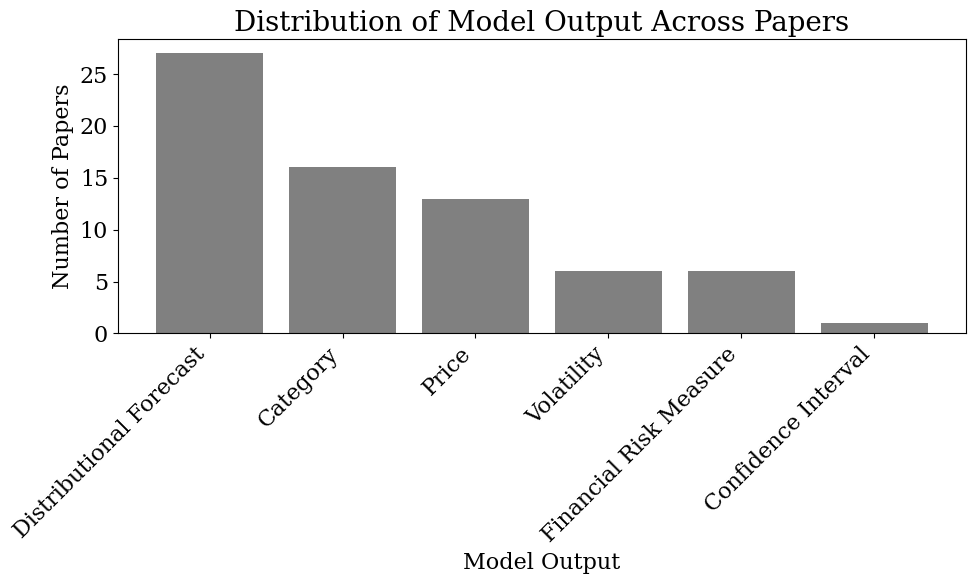
\includegraphics[width=1\linewidth]{Images/model_output.png}
    \caption[Distribution of model output categories in papers]{Distribution of model output categories provided by the models in the papers, with some papers offering multiple outputs.}
    \label{fig:model_output}
\end{figure}

\subsubsection{Price}
13 articles in the sample employ probabilistic AI models to predict asset prices or returns without exploiting the probabilistic models capability to quantify uncertainty.

\textcite{jang2018generative} adopt a Bayesian approach to incorporate prior knowledge about option prices, specifically encoding in the prior that forecasted prices of deep in-the-money (ITM) or out-of-the-money (OTM) options should remain close to their previous prices. Thus, they are able to make better point predictions in situations that differ significantly from the training data, but they do not use the uncertainty estimates.

\textcite{jang2018empirical} use a Bayesian neural network for improved regularization and generalization, outperforming linear regression and Support Vector Regression models for Bitcoin price prediction.

\textcite{choudhury2020enhancing} and \textcite{tang2024period} use Variational Autoencoders (VAEs) as a preprocessing step for LSTM and transformer models, respectively, which in turn generates point predictions for stock prices. By first mapping the input to a lower-dimensional latent space, noise can be reduced, making the regression task easier. \textcite{choudhury2020enhancing} do not mention why a VAE was preferred over a conventional autoencoder (AE). \textcite{tang2024period} suggest that VAEs perform better than AEs for noisy data, but neither their study nor the articles they cite empirically benchmark VAEs against AEs.

In \textcite{Sharma2021}, a clear motivation for the chosen Recurrent Dictionary Learning (RDL) structure is its ability to make predictions with uncertainty, and that a knowledgeable trader may use the uncertainty estimates to make better trading decisions. However, produced uncertainty estimates are not presented or analyzed, and there is no evaluation of whether they in fact are useful.

\textcite{Daniali2021} combine a CNN model with a conditional variance layer. The probabilistic output is not used, but the results show that the proposed model outperforms a traditional CNN in terms of point predictions.

In \textcite{govindasamy2014prediction, li2010stochastic}, predicted probabilities for different states are used to estimate a predicted price without any uncertainty quantification. Both articles outperform benchmarks in terms of point prediction accuracy.

In the other five articles, the authors do not present a clear rationale for using a probabilistic AI model. \textcite{Zmuk2020gpr}, \textcite{Park2014gpr} and \textcite{Papaioannou2022gpr} test several deterministic and Gaussian process regression (GPR) models. Both \textcite{Park2014gpr} and \textcite{Papaioannou2022gpr} show GPR as the best performing model, while in \textcite{Zmuk2020gpr} results are mixed. In \textcite{li2020multivariate}, a VAE is used to ``relief the curse of dimensions'', but the authors do not explain why a \textit{variational} autoencoder is used, rather than a traditional autoencoder. \textcite{salama2024gan} employ a cGAN, only used to generate one sample at prediction time, thus not exploiting the model's ability to predict multiple future scenarios. The accuracy of the point predictions, measured in correlation between predicted returns and actual returns is as high as ~0.999, raising questions about model overfitting or data leakage in the training process.

In conclusion, while the use of probabilistic AI models for point prediction of asset prices may often appear arbitrary, several studies highlight their strong performance. Notably, \textcite{Daniali2021} demonstrate that their probabilistic model outperforms an otherwise identical deterministic counterpart, and \textcite{jang2018generative} exploit Bayesian priors to improve generalization to unseen data.

\subsubsection{Distributional Forecast}
\label{sec:distribution}
There are \distributionaloutput articles in the sample where the proposed model predicts a distribution over future prices. Of these, \distributionalparametric articles involve models outputting flexible distributions, which is beneficial in finance given that financial returns are not normally distributed \parencite{Peir1994TheDO}. The remaining \distributionalnonparametric models assume fixed distributional forms, similar to traditional methods, but retain the advantage of capturing non-linear dependencies.

\textbf{Parametric Distributions}

\distributionalparametric articles use models that output parameters for an assumed distributional form, similar to GARCH predicting variance while requiring an assumed distribution type.

Nine of these articles use Gaussian Process Regression. GPR limits the distributional output to Gaussian forms and cannot by default handle heteroskedastic noise, restricting its utility in financial applications. \textcite{Risk2018gpr} works around this by introducing a conditional variance term in the GPR equation. The output distribution then becomes a combination of one Gaussian distribution representing epistemic uncertainty and one Gaussian distribution representing underlying data uncertainty. This enables portfolio VaR and CVaR estimation with an epistemic confidence interval. The results show that the estimates are of comparable quality to estimates achieved through computationally expensive nested Monte Carlo simulation, where the value of all portfolio assets are calculated for a range of possible economic scenarios. Another example of a GPR model effectively modeling volatility is the local volatility model proposed by \textcite{tegner2021probabilistic}, which explicitly models and predicts the implied volatility surface inferred from option prices.

\textcite{Law2017Practical} employs Bayesian SVR (B-SVR) with explicit error bars incorporating both model-driven (epistemic) uncertainty and intrinsic noise (volatility). However, intrinsic noise is assumed constant across the time series, disregarding financial heteroskedasticity and reducing its utility as an uncertainty measure. The study also lacks validation of uncertainty estimates, though the B-SVR does outperform a traditional SVR in point prediction accuracy. B-SVR's epistemic uncertainty is not distribution-constrained because it is a sum of many distributions—one for each support vector—allowing for flexibility in the output distribution shape. In the paper, however, the practical implementation only considers the variance, removing any non-parametric characteristics.

\textcite{Tian2023} analyze fitting errors to estimate uncertainty and construct prediction intervals, even though the underlying model itself is not probabilistic. These intervals account for both model uncertainty and asset volatility, but have uniform widths across the series, ignoring financial heteroskedasticity and limiting their risk analysis utility.

\textcite{Horenko2020} propose a simple model that is slightly freer in terms of the generated distributions where the user can choose how many moments to output—beyond just mean and variance. The model outperforms GARCH in terms of log likelihood and BIC.

In \textcite{Li2024DeepAR}, the proposed DeepARA model outputs mean and variance, thus predicting both the expected returns and the volatility of stocks, but with an assumed distribution of returns. The usefulness of the uncertainty estimate is not assessed or benchmarked.

\textbf{Non-Parametric Distributions}

The remaining \distributionalnonparametric articles generate non-parametric distributions, allowing arbitrary distribution shapes. Non-parametric distributions are particularly useful for risk analysis, enabling more accurate estimation of measures such as Value at Risk (VaR) or Expected Shortfall (CVaR), given the non-normal distribution of financial returns and frequent extreme events \parencite{Peir1994TheDO}. Several probabilistic AI methods are used to generate these distributions.

Seven articles utilize Bayesian Neural Networks (BNNs), including both feed-forward and recurrent networks \parencite{cocco2021predictions, Hassan2024Bitcoin, Golnari2024Cryptocurrency, soleymani2022longterm, Dixon2022Industrial, chandra2021bayesian, hortua2024forecasting}. As mentioned in Section \ref{sec:bnn}, BNNs model weights as random variables. While the weight distributions often assume normality, the complex interactions of hidden layers and multiple nodes allow for flexible output distributions. However, the uncertainty is primarily tied to model weights rather than data, meaning that the output primarily captures epistemic uncertainty rather than aleatoric uncertainty (volatility). Standard Bayesian estimation techniques also allow for estimating an aleatoric noise term, but only under the assumption of constant variance, which is inadequate for financial time series prediction where volatility changes over time. Nevertheless, it is possible to construct a BNN that also quantifies heteroscedastic aleatoric uncertainty, for instance by predicting variance alongside expected returns and training with appropriate loss functions, but such an approach is only explored by \textcite{hortua2024forecasting} and \textcite{soleymani2022longterm}. Consequently, although many authors assert that predicted uncertainty aids investment decisions, most models in this category are inadequate for financial risk analysis, as the uncertainty estimates reflect model unfamiliarity rather than intrinsic asset risk. The extended models that quantify aleatoric uncertainty, however, are of particular interest.

\textcite{eriolu2020bootstrapped} employ bootstrapping to generate non-parametric confidence intervals, but ignore heteroscedasticity and the coverage probability of the produced confidence intervals is off by 55 percentage points.

As noted earlier, GPR models are typically limited to parametric Gaussian output distributions and assume homoskedastic noise. \textcite{Platanios2014gpr} overcome these constraints by incorporating heteroskedastic noise into the GPR framework and employing a Pitman-Yor process to integrate a potentially infinite set of GPR models, enabling the modeling of highly complex distributions. Despite these advancements, the authors do not explicitly analyze the shape of the resulting distributions. However, they demonstrate that the volatility estimates produced by their model align more closely with squared returns than those of GARCH. Their stock index modeling experiment with data from 1993 to 2003 shows a reduction to roughly one-tenth of GARCH's RMSE, while the forex experiment and the experiment on newer stock index data exhibit notable, though less extreme, improvements. Unfortunately, they do not test for significance or measure and benchmark other relevant metrics such as coverage probability.

\textcite{arian2022encoded} employ a VAE to generate return samples for each stock in a portfolio, preserving correlations between assets. This is achieved by repeatedly sampling from the random variables in the latent space and passing these samples through the deterministic decoder part of the network. These samples can be used to construct non-parametric distributions for both individual assets and portfolio returns. From these distributions, the authors calculate VaR for three portfolios, outperforming traditional models in scoring functions, but failing Christoffersen's test for adequacy.

\textcite{Fatouros2023DeepVaR} and \textcite{Almeida2024RiskForecasting} apply DeepAR to model asset and portfolio returns. DeepAR, inherently a multi-series model, outputs expected return and volatility for each asset, assuming a distributional form. However, the authors generate samples for portfolio returns where each sample includes simulated returns for every stock in the portfolio. This sampling process allows the construction of non-parametric distributions for the portfolio returns. \textcite{Fatouros2023DeepVaR} show that the proposed model for forex portfolio VaR estimation passes both Christoffersen's conditional coverage test and the Dynamic Quantile (DQ) test. Additionally, it outperforms a diverse set of appropriate baseline models, such as GARCH, RiskMetrics (RM), Bidirectional Generative
Adversarial Networks (BiGAN), Historical Simulation (HS) and the Monte Carlo method. The proposed model by \textcite{Almeida2024RiskForecasting} for cryptocurrency VaR and CVaR estimation is also extensively tested, but the results show that it is consistently outperformed by GARCH.

\textcite{lee2021estimation} and \textcite{vuletic2024finGAN} employ conditional Generative Adversarial Networks (cGAN) to forecast prices of stocks and stock indices. By inputting recent returns alongside generated noise vectors into the cGAN, they produce samples representing diverse future scenarios, thereby forming a non-parametric distribution. Similarly, \textcite{Park2024UncertaintyAware} use reinforcement learning and quantile regression to construct non-parametric distributions. However, all articles focus solely on the standard deviations of produced distributions, overlooking other potentially informative properties. Nonetheless, the meaningfulness of the uncertainty estimates is demonstrated by comparing the performance of trading strategies where the predicted standard deviations are taken into account to simpler strategies. However, informativeness of their uncertainty estimate is not assessed using e.g. Christoffersen's test, and neither is it benchmarked against traditional models such as GARCH.

Finally, \textcite{wang2020fastconformal} apply a Conformal Predictive System (CPS) with a regularized extreme learning machine to produce non-parametric cumulative distribution functions (CDFs) of returns. Though not benchmarked against other models, the generated predictions appear reliable, with the observed quantiles closely matching expected frequencies.

\textbf{Conclusion on Distributional Forecasts}

Most parametric distribution models provide uncertainty quantification primarily of the model itself, rather than the underlying data, limiting relevance for financial risk assessment. Only the models proposed by \textcite{Risk2018gpr} and \textcite{Horenko2020} offer parametric distributions with potential financial interpretations, with \textcite{Horenko2020} demonstrating superior performance over GARCH.

In the non-parametric category, all models, except most of the Bayesian Neural Networks (BNNs), yield distributions with potential implications for risk management. However, most either fail to pass relevant tests or lack sufficient rigorous evaluation to confirm superiority over traditional risk modeling methods. The notable exception is the DeepAR model by \textcite{Fatouros2023DeepVaR} for forex VaR estimation, which undergo extensive testing with favorable results. Additionally, the DeepAR model can model multiple assets simultaneously, accounting for their correlations.

\subsubsection{Confidence Interval}

\textcite{Wang2024GoldForecasting} presents a model that directly outputs a confidence interval for future gold prices, rather than a point estimate or distributional forecast. This is achieved by using a LSTM variant outputting a lower and upper bound for the confidence interval, trained using quantile loss. Results yield high coverage, meaning actual values end up within the predicted intervals at least as often as expected. However, absence of benchmark comparisons—e.g. against traditional models like GARCH—makes it difficult to conclude whether the high coverage reflects accurate forecasting or simply wide intervals.


%----------------Volatility-----------------------%

\subsubsection{Volatility}

While volatility can be inferred from the probabilistic outputs of some models discussed in \ref{sec:distribution}, \volatilityoutput articles in the sample explicitly predict volatility or its proxies.

Three articles—\textcite{xing2019sentiment}, \textcite{Parker2021BayesianHeteroskedastic} and \textcite{Platanios2014gpr}—attempt to model latent, unobservable volatility directly, without relying on proxies. 

\textcite{xing2019sentiment} achieves this by using a negative ELBO loss function to train a proposed hybrid model, combining a VAE and a RNN with sentiment data. Theoretically, minimizing the negative ELBO enables the model to make optimal predictions for latent volatility. Model performance is evaluated through negative log-likelihood (NLL) and compared against traditional models like GARCH variants and other machine learning methods, showing consistent outperformance. Statistical tests are also conducted to assess wether the outperformance is significant, displaying strong evidence against other machine learning models, but weak evidence against GARCH, and no evidence against modified GARCH models.

\textcite{Parker2021BayesianHeteroskedastic} argue that the proposed Echo State Volatility Model (ESVM) provides better volatility estimates than GARCH. However, as mentioned in Section \ref{sec:prob_rnn} is is difficult to assess whether this result is reliable.

\textcite{Platanios2014gpr} estimate volatility using a complex non-parametric distribution derived from GPR models, as detailed in Section \ref{sec:distribution}. In these models, volatility is treated as heteroskedastic noise, similar to GARCH, but with seemingly higher accuracy in terms of RMSE against squared returns.

The remaining five articles predict various observable proxies for volatility. \textcite{tegner2021probabilistic} predict the ``implied volatility surface''—that is, the implied volatility based on prices for options with different strike prices and different maturity dates—and show superior performance compared to a naive forecast. It is unclear which proxy \textcite{jang2018empirical} predicts, but it appears to be a proxy, considering that they are using RMSE to compare predictions with ``true values''. \textcite{Daniali2021} use a CNN to predict the VIX, while \textcite{Tian2023} use a RNN-based model to predict several volatility indices, outperforming a diverse set of benchmark models, including ARIMA and various neural networks. Lastly, \textcite{Hocht2024gpr} use a GPR to predict realized volatility with the purpose of pricing complex options.

In conclusion, the models proposed by \textcite{tegner2021probabilistic}, \textcite{xing2019sentiment}, and \textcite{Platanios2014gpr} appear promising, demonstrating potential superiority over traditional models, though their evaluation methodology could be more exhaustive. \textcite{Parker2021BayesianHeteroskedastic} also claim to outperform GARCH; however, the reported metrics raise concerns about the fairness of the comparison.


%--------------------Financial risk measures----------------------%

\subsubsection{Financial Risk Measures}
\label{sec:financial_risk_measures}

Many articles in Section \ref{sec:distribution} produce uncertainty distributions that can be utilized to calculate financial risk measures like Value at Risk (VaR) or Conditional Value at Risk (CVaR). However, only six articles in the sample explicitly aim to produce risk measures.

Five of these estimate VaR or CVaR from model generated uncertainty distributions. The remaining article, \textcite{caprioli2023quantifying}, employs a distinct method using a VAE to generate synthetic correlation matrices as inputs for VaR calculation. Instead of deriving VaR from a single observed distribution, the VAE samples multiple plausible correlation structures to represent various market conditions. These correlation matrices are then used in a Monte Carlo simulation within a multi-factor Vasicek model to derive a distribution of portfolio losses to calcualte VaR.

Although there are six articles making VaR predictions, their approaches to evaluating the correctness of these predictions vary.

The most straightforward method to assess prediction intervals and VaR estimates is to verify whether the frequency of violations—i.e., the occurrence of data points exceeding the predicted VaR—matches the chosen significance level. For instance, with a VaR estimate at a 5\% significance level, approximately 5\% of observed values should lie outside the predicted range. Over the short term, discrepancies may arise, but in the long term this should hold. This property can be statistically tested via an unconditional coverage test, commonly referred to as Kupiec's test \parencite{kupiec1995techniques}. \textcite{Fatouros2023DeepVaR} and \textcite{arian2022encoded} both pass this test, even when GARCH models do not. \textcite{Horenko2020} also reference Kupiec and report VaR violation frequencies, though the absence of p-values makes it unclear if the model passes the test. In the other three articles, no such test is conducted \parencite{Almeida2024RiskForecasting, Risk2018gpr, caprioli2023quantifying}.

For heteroscedastic time series, verifying only that the violation frequency matches the expected proportion is inadequate, as volatility in financial time series is time-varying. VaR estimates must vary correspondingly. A model predicting constant VaR could pass the unconditional coverage test, yet still be inadequate. To address this, \textcite{Christoffersen1998} proposed a conditional coverage test evaluating whether VaR violations are independent across time. Models making constant VaR predictions typically fail this test due to clusters of violations in periods of high volatility. Only \textcite{Fatouros2023DeepVaR} and \textcite{arian2022encoded} conduct the conditional coverage test, also known as Christoffersen's test, and the model in \textcite{arian2022encoded} fails.

Testing CVaR estimates is more complex, but several tests, such as the Acerbi and Szekely \parencite{acerbi2014backtesting} test and the Du and Escanciano test \parencite{Du2017}, have been developed. However, neither of the two articles that estimate CVaR apply these tests; instead, they rely on scoring functions for evaluation. \textcite{Risk2018gpr} assess CVaR using RMSE against Harrell-Davis estimates as a proxy for the ``ground truth,'' without benchmarking against traditional models. \textcite{Almeida2024RiskForecasting} use the Continuous Ranked Probability Score (CRPS) and demonstrate superiority relative to GARCH.

Additionally, to demonstrate that a VaR or CVaR model is an improvement over traditional approaches, appropriate scoring functions and benchmarking are essential. All six articles employ scoring functions, yet only four benchmark their models against traditional ones, with only \textcite{Fatouros2023DeepVaR} and \textcite{Horenko2020} demonstrating clear superiority.




%-----------------------Categorization -------------------------%

\subsubsection{Categorization}
Sixteen articles in the sample propose classification-based models for financial forecasting, targeting variables such as price direction (e.g., rise or fall) rather than precise future price levels. Prior research indicates that forecasting direction yields better investment returns, as trading success depends on correctly anticipating price movement rather than exact price levels, where small estimation errors can cause significant trading mistakes \parencite{Enke2005}. Additionally, models providing probabilistic forecasts (e.g., a 54\% probability of a price increase) enhance interpretability by explicitly conveying the uncertainty associated with predictions.

Most machine learning classification models can output class probabilities, but these probabilities are often poorly calibrated, which means that the estimated probabilities do not match the true class proportions \parencite{guo2017calibration, NiculescuMizil2005}. If that is the case, the predictions lose their interpretability, and the probabilities provide little insight. Thus, this review only includes classification models that are based on probability theory.

Some of the most commonly used models for classification in the sample includes Hidden Markov Models \parencite{sher2023exploiting, park2011trend, zhang2019high, su2022hmm,cao2019multi}, Bayesian Neural Networks \parencite{Malagrino2018Forecasting, magris2023bayesian} and Probabilistic Neural Networks \parencite{Thawornwong2004pnn, Lahmiri2024pnn, Chandrasekara2019pnn}.

Although most proposed classification models in the sample have the potential to produce well-calibrated probabilities, few articles assess whether the probabilities are actually well-calibrated. Even with a model based on probability theory, it is possible to end up with distorted class probabilities, e.g. if the model is misspecified or biased. An exception is \textcite{magris2023bayesian}, where the probabilities are thoroughly assessed using Expected Calibration Error (ECE) and Expected Calibration Distance (ECD). Of these two, ECD is the more robust metric, because it measures the distance between the predicted probability distribution and the empirical distribution, rather than just comparing the average difference between predicted probabilities and actual outcomes grouped into intervals (called bins), as ECE does. Thus, ECD is less sensitive to localized performance spikes.

A drawback of using a classification model instead of a price level model is that the aleatoric uncertainty estimate will no longer correspond to volatility—i.e. the standard deviation of the price—which makes it less comparable to other risk models, and prevents the calculation of financial risk measures such as Value-at-Risk. However, \textcite{kim2023portfolio} construct a risk measure based on the uncertainty of the classification predictions and show that it is useful for portfolio management.


%---------------------Conclusion----------------------%
\subsubsection{Conclusion} % deside if we need this
Table \ref{table:conclusions_by_target_variable} summarizes the key findings for each type of model output. In short, the results show that probabilistic AI can be useful for every type of output, with non-parametric distributions having especially interesting use cases. However, many articles do not provide an appropriate interpretation of the probabilistic output, and the motivation for using probabilistic AI is not always clear.


\begin{table}[H]
    \centering
    \caption[Summarizing Conclusions by Model Output]{Summarizing Conclusions by Model Output.}
    \label{table:conclusions_by_target_variable}
    \small
    \begin{adjustbox}{width=0.5\textwidth,center}
    \begin{tabular}{p{0.1\textwidth}p{0.40\textwidth}}
        \toprule
        \textbf{Target Variable} & \textbf{Conclusion} \\
        \midrule
        Price & \smallbullet{Often unclear why a probabilistic model is used to make point predictions for price} \smallbullet{Some studies show outperformance compared to deterministic models} \\
        \addlinespace
        \hdashline[0.2pt/3pt]
        \addlinespace
        Distributional forcast & \smallbullet{Flexible, non-parametric models can enhance risk estimation by capturing non-linear dependencies and diverse distributional shapes. However, most either fail to pass relevant tests or lack rigorous evaluation to confirm superiority over traditional risk modeling methods} \smallbullet{Most parametric distribution models provide uncertainty quantification primarily of the model itself, rather than the underlying data, limiting their relevance for financial risk assessment } \\
        \addlinespace
        \hdashline[0.2pt/3pt]
        \addlinespace
       Confidence interval & \smallbullet{Only one paper suggest a model outputting confidence interval—a LSTM variant with high coverage, but absence of benchmark comparisons limits the evaluation of forecast accuracy} \\
        \addlinespace
        \hdashline[0.2pt/3pt]
        \addlinespace
        Volatility & \smallbullet{Mixed results on performance against traditional models: some non-parametric models show promise, in particularly in heteroskedasticity modeling} \smallbullet{Limited benchmarking against e.g. GARCH makes it difficult to validate claims of model superiority} \\
        \addlinespace
        \hdashline[0.2pt/3pt]
        \addlinespace
        Financial risk measures & \smallbullet{Many papers produce distributions that can be utilized to calculate financial risk measures, but only a few papers create models that explicitly aim to produce VaR or CVaR; most lack rigorous statistical test to validate results} \smallbullet{Several scoring metrics are used, but few benchmark against traditional models} \\
        \addlinespace
        \hdashline[0.2pt/3pt]
        \addlinespace
        Categorization & \smallbullet{Main focus on forecasting price movements. Sample included models that produce well-calibrated probabilities, but lack differentiation between epistemic and aleatoric uncertainty, limiting use for modeling asset volatility} \smallbullet{Models support human interpretability and portfolio construction due to well-calibrated probabilities, but offer minimal insights into inherent risk} \\
        \addlinespace
        \addlinespace
        \bottomrule
    \end{tabular}
    \end{adjustbox}
\end{table}





%----------------------------------------------------%
% --------- Analysis by Asset -----------------------%
%----------------------------------------------------%

\subsection{Analysis by Asset Class}
\label{sec:analysis_by_asset}
The motivations for making predictions and quantifying uncertainty, as well as the feasibility of doing so, can vary among asset classes. In the following section, we provide an overview of how probabilistic AI has been applied to different asset classes, examining the purposes it serves and the specific challenges encountered in each case. Figure \ref{fig:asset_type_predicted} illustrates the frequency each asset class the proposed models in our sample is trained to predict. Results and conclusions by asset classes are summarized in Table \ref{table:conclusions_by_asset_classes}.

\begin{figure}[H]
    \centering
    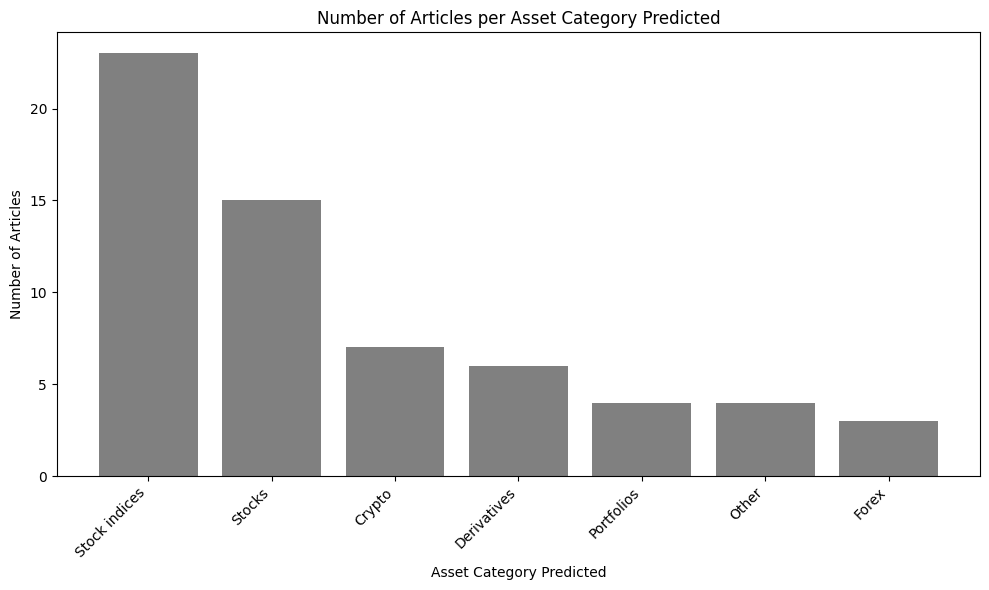
\includegraphics[width=1\linewidth]{Images/articles_per_asset_type_predicted.png}
    \caption[Distribution of asset categories predicted across papers]{Asset type predicted across papers.}
    \label{fig:asset_type_predicted}
\end{figure}
\makeatletter


% --------- Stocks -------------------------------%
\subsubsection{Stocks}
Individual stocks are predicted in \stockarticles articles. While a few studies focus on a single stock, the majority apply a common model to multiple. Accurately predicting stock prices has proven challenging due to market efficiency \parencite{fama1970efficient}, which posits that prices fully incorporate all available information. In contrast, volatility has demonstrated greater predictability \parencite{poon2003forecasting}, emphasizing the relevance of uncertainty estimation for stocks. 

Most authors do not explicitly state distinct motivations for constructing uncertainty estimates using probabilistic AI. Instead, focus tend to be on achieving accurate price or return predictions to develop trading strategies or inform investor decisions, with uncertainty estimates often presented as a secondary feature beneficial for risk management. Trading strategies rely on informed beliefs about future price movements \parencite{vuletic2024finGAN}, and accurate range predictions are valuable for risk management \parencite{Li2024DeepAR}, as improved uncertainty estimates can help investors make more informed decisions. \textcite{govindasamy2014prediction} note that the main problem faced by investors is that they do not have a clear idea on what stocks to invest in to maximize profits.  

Some studies examine how external factors impact the uncertainty of individual stocks across countries and sectors differently \parencite{chandra2021bayesian, soleymani2022longterm}. Notably, \textcite{chandra2021bayesian} select stocks from multiple countries to analyze the COVID-19 pandemic's effect on stock price fluctuations, highlighting the varying impact of global events on asset-level uncertainty and underscoring the need for robust uncertainty quantification. 

% --------- Stock Indices-------------------------%
\subsubsection{Stock Indices}
Stock indices are tied as the most commonly predicted asset, featured in \stockindexarticles articles, with strong focus on American, European and Asian indices. Since indices are typically composed by multiple stocks from different sectors, they are generally less volatile than individual stocks and more indicative of the general state of the economy \parencite{sezer2020financial}. Therefore, uncertainty quantification can provide valuable insight into underlying market volatility. 

Most authors primarily focus on the trading applications of accurately forecasting indices, but a subset of researchers emphasize the possibility of underlying market investigation. \textcite{Suphawan2022gpr} note that stock indices reflect the market, and reliable uncertainty estimates are therefore valuable in financial decision-making and risk management. \textcite{Wang2021gprensemble} state that accurate forecasts of index fluctuation characteristics can aide government departments in timely and effectively supervising and guiding the market to avoid financial risk. In addition, with the globalization of the world economy, two studies investigate interdependencies between indices across the world \parencite{cao2019multi, Malagrino2018Forecasting}, motivated by uncertainty estimates' importance to support risk management strategies on international scale.

% --------- Portfolios --------------------------%
\subsubsection{Portfolios}
Among the nine articles in the sample focusing on portfolios, where authors explicitly construct asset combinations and forecast value, returns or risk measures, the predominant motivation is to maximize portfolio returns while integrating financial risk measures to assess and manage uncertainty. As a result, articles in this category often genuinely care about risk. In addition, \textcite{Risk2018gpr} actualize regulatory compliance with Solvency II requirements within insurance for risk assessment at the 99.5\% confidence-level. \textcite{kim2023portfolio} emphasize the motivation for using probabilistic models with distributional outputs over deterministic models, as the variance of predicted distributions can signify uncertainty, enabling simultaneous maximization of returns and minimization of risk. Most studies derive quantile-based risk measures from distributional outputs, with \textcite{Fatouros2023DeepVaR, arian2022encoded, caprioli2023quantifying} focusing on VaR, and \textcite{Risk2018gpr, Min2023BlackLitterman} also estimate CVaR.

% --------- Crypto -----------------------------%
\subsubsection{Cryptocurrencies}
There are \cryptoarticles articles in the sample forecasting cryptocurrencies, with Bitcoin being the most prevalent. Recent studies of the most frequently traded cryptocurrencies suggest that the markets are becoming increasingly efficient and interconnected, although efficiency and volatility can fluctuate over time \parencite{noda2021evolution, liu2019volatility, gupta2022empirical}. Increasing adaptation and acceptance of cryptocurrencies has led investment to become increasingly common, and fostered a growing need to understand the nature of volatility in cryptocurrency \parencite{gupta2022empirical}.

Most researches are motivated by the largely fluctuating prices and its implications for risk management. \textcite{Golnari2024Cryptocurrency} note that rapid value fluctuations make accurate prediction challenging and emphasize that understanding the inherent uncertainty in predictions and price dynamics is crucial for effective risk management in investment and trading. Similarly, 
\textcite{Almeida2024RiskForecasting} highlight the substantial loss potential in crypto markets, underscoring the importance of understanding risk and implementing effective risk management strategies. \textcite{cocco2021predictions} state that the high volatility of cryptocurrencies has made trading highly relevant in recent years, and suggest that speculation may be profitable. 


% --------- Forex -----------------------------%
\subsubsection{Forex}
Foreign exchange (forex) represents one of the most liquid and interconnected asset classes, influenced by several macroeconomic factors, geopolitical dynamics and international trade, making uncertainty quantification challenging \parencite{Rossi2013ExchangeRP}. \forexarticles articles in the sample forecast forex rates, usually just as one of many model applications studied \parencite{park2011trend, Platanios2014gpr, tang2024period, li2010stochastic, Papaioannou2022gpr}. As a result, explicit motivations for developing uncertainty estimates specific to forex forecasting is limited. However, \textcite{cao2019multi} highlight the importance of investigating cross-market influences, such as interaction between forex and stock markets, for international risk management, and uncertainty estimates as a way to understand the forex market's response to global market dynamics.

% --------- Derivatives -----------------------%
\subsubsection{Derivatives}
Derivatives are financial instruments whose value are derived from an underlying asset, such as stocks, bonds or indices. Since derivatives are commonly priced based on uncertainty in potential outcomes from the underlying assets behavior, improving uncertainty estimates can potentially reveal arbitrage opportunities \parencite{black_scholes_1973}. \derivativesarticles articles focus on derivatives. 

A common derivative in the sample are volatility indices, where \textcite{hortua2024forecasting, Daniali2021} analyze the VIX, while \textcite{Tian2023} extend their analysis to include the COEVI and TYVIX. \textcite{hortua2024forecasting} note that volatility indices, and the VIX in particular, are recognized as good indicators of investor sentiment and market turbulence, making it valuable for asset managers and regulators to foresee, but that it remains difficult to forecast. Probabilistic forecasts of these indices could therefore be valuable to quantify the uncertainty around future volatility, and achieve more adequate financial inference.

Options are another commonly studied derivative, with \textcite{Park2014gpr} analyzing KOSPI options, \textcite{DeSpiegeleer2018gpr} S\&P options and \textcite{tang2024period} different ETF options. \textcite{Park2014gpr} highlight a key limitation of traditional models like Black-Scholes: their inability to provide predictive distributions of the option prices. Probabilistic models, such as the GPR employed in their study address this gap, which the authors claim improve risk assessment—a primary motivation in the study. 

Lastly, the sample include studies on credit default swap spreads \parencite{Law2017Practical} and capped volatility swaps \parencite{Hocht2024gpr}. 


\subsubsection{Commodities}
\commoditiesarticles articles in the sample predict commodities.
\textcite{Wang2024GoldForecasting} forecast gold prices, and advocate the need for a probabilistic framework under extreme uncertainty. The authors argue that point estimates are insufficient in such conditions, whereas interval predictions provide meaningful insights for managing uncertainty. Gold's important position in the global economy is also pointed out, underscoring the need for robust predictive models that incorporate uncertainty to improve risk assessment. \textcite{Law2017Practical} predict gold and crude oil prices among a range of other assets, but do not discuss underlying motivations. \textcite{li2020multivariate} forecast soybean futures, emphasizing the importance of accurate predictions and uncertainty quantification to facilitate decision making in agriculture risk management and crop insurance programs, vital for policymakers and investors. They also underscore that assumptions of independent variables and normal distributions commonly enforced by traditional models do not align with the real market conditions for commodities.


\subsubsection{Bonds}
\textcite{Law2017Practical} predict various financial assets, including both US 10-year Treasury and UK Gilt 10-year bond yields. They do not discuss motivation for using a probabilistic framework for predicting the bond yields specifically. 



% --------- Conclusion -----------------------%


% Write that we dont assess bonds.  

\subsubsection{Conclusion} % deside if we need this

Table \ref{table:conclusions_by_asset_classes} summarizes the primary focus and motivations of the authors making uncertainty estimates for the studied asset classes. Most authors do not exhibit clear motivations specific to asset type predicted, but common themes include enhanced financial decision making, support for trading purposes and risk management. An exception is the portfolio category, where authors genuinely have an underlying motivation of assessing risk. Several authors predict multiple asset classes, and do not describe distinct motivations beyond demonstrating model applicability in diverse contexts. 

\begin{table}[H]
    \centering
    \caption[Summarizing Conclusions by Asset Classes]{Summarizing Conclusions by Asset Classes.}
    \label{table:conclusions_by_asset_classes}
    \small
    \begin{adjustbox}{width=0.5\textwidth,center}
    \begin{tabular}{p{0.1\textwidth}p{0.40\textwidth}}
        \toprule
        \textbf{Asset Class} & \textbf{Conclusion} \\
        \midrule
        Stocks & \smallbullet{Utilize probabilistic forecasts for better trading and risk management} \smallbullet{Quantify how external factors impact stock uncertainty across markets} \\
        \addlinespace
        \hdashline[0.2pt/3pt]
        \addlinespace
        Stock indices & \smallbullet{Index uncertainty can reflect broader market volatility, aiding in financial decision-making} \smallbullet{Understanding interdependencies between international indices to enhance cross-border risk management} \\
        \addlinespace
        \hdashline[0.2pt/3pt]
        \addlinespace
        Portfolios & \smallbullet{Maximizing portfolio returns while leveraging uncertainty estimates for risk management} \smallbullet{Probabilistic models provide distributional outputs that can be used to create risk measures like VaR} \\
        \addlinespace
        \hdashline[0.2pt/3pt]
        \addlinespace
        Crypto & \smallbullet{High volatility of cryptocurrencies underscore need for uncertainty quantification in risk-aware trading and investment} \smallbullet{Understanding fluctuating market dynamics for managing potential losses and leverage speculative opportunities} \\
        \addlinespace
        \hdashline[0.2pt/3pt]
        \addlinespace
        Forex & \smallbullet{Highly interconnected asset making uncertainty quantification important for international risk and trade management} \smallbullet{Often predicted as one of many time series without explicit motivations} \\
        \addlinespace
        \hdashline[0.2pt/3pt]
        \addlinespace
        Derivatives & \smallbullet{Probabilistic models address limitations of traditional methods providing predictive distributions} \smallbullet{Volatility indices and option studies most prevalent} \\
        \addlinespace
        \hdashline[0.2pt/3pt]
        \addlinespace
        Commodities & \smallbullet{Uncertainty estimation important for informed decision making in e.g. agriculture risk management and global gold price influence} \smallbullet{Probabilistic models can address distribution assumptions enforced by traditional models that do not align with commodity markets}  \\
        \addlinespace
        \hdashline[0.2pt/3pt]
        \addlinespace
        Bonds & \smallbullet{Only one paper in the sample predicts bonds}  \\
        \addlinespace
        \addlinespace
        \bottomrule
    \end{tabular}
    \end{adjustbox}
\end{table}



%----------------------------------------------------%
% --------- Analysis by Type of Uncertainty-----------%
%----------------------------------------------------%

%Remember to include somehow the measures/how autors assess their uncertainty estimate—we also need to evaulate the strenght of these estimates, but that might be conclusion %


\subsection{Analysis by Type of Uncertainty}
\label{sec:analysis_by_type_of_uncertainty}

All models in the sample are capable of providing predictions with quantified uncertainty, but the type of uncertainty and how the authors interpret it vary significantly. Shown in Figure \ref{fig:uncertainty_quantification_by_type_and_assessment}, many authors neither use nor interpret the uncertainty estimates at all. When uncertainty estimates are presented, authors usually treat them as total uncertainty, without assessing whether it arises from modeling limitations (epistemic uncertainty) or from the inherent volatility of the underlying asset (aleatoric uncertainty). This distinction is crucial for investment decisions because it is important to know whether the uncertainty is due to an unreliable model or a risky asset.

Furthermore, only a minority of articles evaluate the quality and usefulness of the uncertainty estimates, and even fewer compare these estimates against traditional models. The following sections explore the various ways uncertainty quantification has been used in the sample articles, the financial relevance of each type of uncertainty, and how different uncertainty estimates have been and can be assessed. Summarizing results and conclusions by type of uncertainty are depicted in Table \ref{table:conclusions_by_uncertainty}.


\begin{figure}[H]
    \centering
    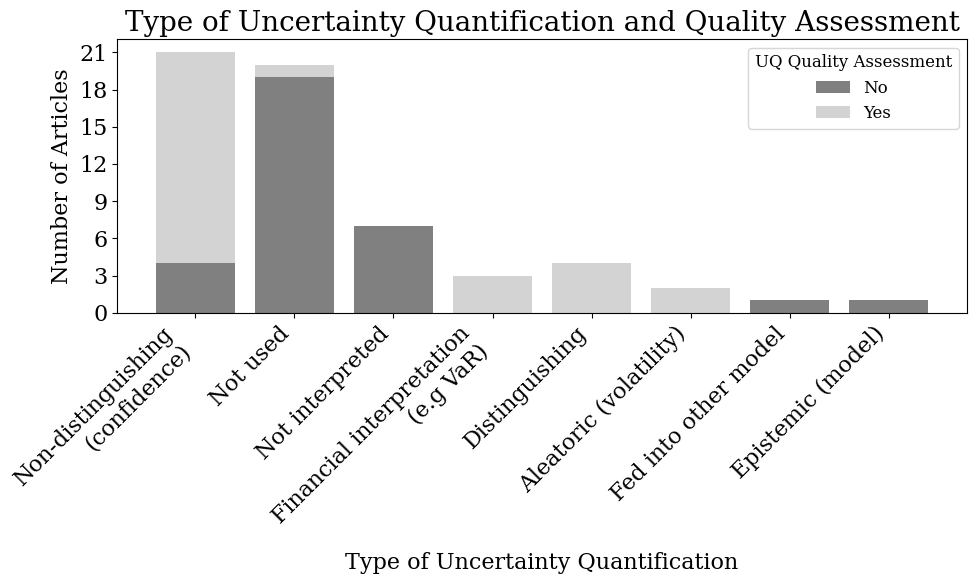
\includegraphics[width=1\linewidth]{Images/uncertainty_quantification_by_type_and_assessment.png}
    \caption[Breakdown of authors’ interpretation and quality assessment of uncertainty estimates]{Authors' interpretation of the uncertainty estimates generated by the models and whether the correctness of these uncertainty estimates was assessed.}
    \label{fig:uncertainty_quantification_by_type_and_assessment}
\end{figure}


%--------------------Not Interpreted or not used-------------------------%
\subsubsection{Not Used}

Among the \samplesize articles in the sample, \uqnotused do not in any way mention or illustrate that their models can produce outputs with uncertainty, even though the utilized model inherently have the capability. In most cases, the authors' motivations for using probabilistic models are not clear, but some show that a probabilistic model can produce better point estimates \parencite{Daniali2021, Papaioannou2022gpr, Park2014gpr}, while others apply probabilistic principles to improve generalization \parencite{jang2018generative}.

\subsubsection{Not Interpreted}

In \uqnotinterpreted articles, the probabilistic outputs from the model are presented, but not interpreted or assigned any financial or technical meaning. Generally, this is simply because the authors do not focus on uncertainty estimation, but rather accuracy of point predictions (e.g. \cite{DeSpiegeleer2018gpr}), or accuracy of category classifications (e.g. \cite{Malagrino2018Forecasting, Zhang2016}).


%-----------------------Epistemic-----------------------------%
\subsubsection{Epistemic (model-uncertainty)}
Epistemic uncertainty arises from uncertainty about which model to use or whether the estimated parameters are correct. Typical causes for this include a lack of enough data or omitted features \parencite{hullermeier2021aleatoric}.

\textcite{Hassan2024Bitcoin} is the only paper interpreting the quantified uncertainty as purely epistemic, with the proposed Bayesian LSTM model tasked with predicting Bitcoin price. Specifically, Monte Carlo dropout is used to estimate the LSTM weights—a Bayesian inference technique introduced by \textcite{gal_ghahramani_2015}. This technique involves keeping dropout active during prediction time, allowing the model to generate as many predictions as desired. These predictions form a distribution that captures the model's uncertainty about which weights are optimal. By default, this approach estimates only epistemic uncertainty, without capturing latent volatility or providing a total uncertainty estimate, unless specifically designed to do so.

As with other uncertainty estimates, it is possible to test the adequacy of epistemic uncertainty estimates by constructing confidence intervals and examining the coverage, but such tests are not conducted in the article.


%-------------------Aleatoric-------------------------------%
\subsubsection{Aleatoric (volatility)}
There are only \uqaleatoric articles in the sample that interprets the quantified uncertainty as exclusively aleatoric, meaning underlying data uncertainty, which in finance is referred to as latent volatility. This is of major interest within finance, as it is the primary measure for risk, and often the basis for deriving other risk measures \parencite{Brooks2003VolatilityFF}.

Two of the articles in the sample \parencite{arian2022encoded, xing2019sentiment} do this through the use of Variational Auto-Encoders (VAE), that can generate non-parametric output distributions through repeated sampling, thereby capturing a spectrum of potential future scenarios, as described in Section \ref{sec:distribution}.

The two other articles use Quantile Regression Deep Learning \parencite{Wang2024GoldForecasting} that quantifies aleatoric uncertainty through estimating several quantiles of the underlying distribution, and MaxEnt-modeling which is an application of the maximum entropy principle \parencite{Horenko2020}.

Testing the quality of aleatoric uncertainty estimates can be conducted similar to testing the quality of financial risk measures in Section \ref{sec:financial_risk_measures}. It should be ensured that the model on average produces uncertainty estimates of the correct magnitude (coverage testing) and that it is able to capture the heteroscedasticity of financial time series (conditional coverage testing). Additionally, it is useful to assess performance relative to traditional models using scoring metrics such as coverage relative to width, negative log-likelihood (NLL), and interval scores.

All four mentioned articles apply relevant scoring metrics and all except \textcite{Wang2024GoldForecasting} compare their results to GARCH and similar models. However, only \textcite{arian2022encoded} and \textcite{Horenko2020} conduct statistical tests for adequacy, which they unfortunately do not pass.

Some of the models that will be discussed in Section \ref{sec:total_uncertainty} below also use techniques that can capture aleatoric uncertainty, but they do not quantify it separately from the epistemic uncertainty.

%-----------------------Total uncertainty--------------------------%

\subsubsection{Total Uncertainty (non-distinguishing)}
\label{sec:total_uncertainty}

Out of the \uqanyinterpretation articles where the authors interpret uncertainty, the majority (\uqnondisting) treat it as total uncertainty. In this context, the uncertainty is supposed to indicate how likely it is that the prediction is accurate. However, authors fail to identify the sources of uncertainty—epistemic and aleatoric—and it remains unclear how much uncertainty comes from each source. Authors often state that knowing the model's confidence in its predictions is useful in investment decisions. However, not distinguishing between aleatoric and epistemic uncertainty limits the models' usefulness, because investors cannot determine whether the uncertainty stems from the inherent riskiness of the predicted assets or from a poor model fit.

Additionally, many authors use uncertainty quantification techniques that are unsuitable for determining total uncertainty in financial time series prediction. For example, six articles in this category employ probabilistic AI models based on Bayesian methods \parencite{Law2017Practical,cocco2021predictions,Golnari2024Cryptocurrency,Dixon2022Industrial,chandra2021bayesian,magris2023bayesian}. While Bayesian models can be used to estimate both epistemic and aleatoric uncertainty, they typically require making assumptions about the aleatoric noise, such as assuming it is normally distributed with a constant variance. As a result, these models are not ideal for capturing uncertainty in financial time series, where latent volatility changes over time. To address this limitation, models must be explicitly designed to account for such dynamics—for instance, by constructing a Bayesian neural network that predicts both an expected price and a variance. None of the six mentioned articles takes such an approach.

One possible explanation for this modeling flaw is that most articles are authored by researchers from computer science rather than finance disciplines (see Figure \ref{fig:author_faculty_origin}). As a result, they may overlook the importance of heteroskedastic noise in finance. Another explanation is that, despite the use of probabilistic AI, many studies focus primarily on the accuracy of their point predictions, treating uncertainty estimates as extra benefits of their modeling approach. This hypothesis is supported by the minimal discussion of uncertainty estimates in many articles.

Among the articles in this category where the uncertainty estimates have been evaluated, assessment typically involves coverage probabilities or portfolio performance when incorporating these estimates (see Table \ref{table:evaluation_criteria}). While both these testing approaches are informative, they are insufficient to conclude on the practical utility of these uncertainty measures in finance. Coverage probability alone overlooks heteroscedasticity \parencite{Christoffersen1998}, while portfolio performance is sensitive to random events when evaluated over a limited time period \parencite{barras2010}.

Models quantifying total uncertainty can be compared using metrics like coverage and uncertainty magnitude. However, absence of comparable traditional econometric models complicates the evaluation of their contributions to the field. Among the \uqnondisting articles in this category, only \textcite{Platanios2014gpr} compares total uncertainty estimates to GARCH. Although superior RMSE against squared returns is reported, this comparison may be inappropriate, as minimizing RMSE against squared returns is not the primary objective of GARCH \parencite{BOLLERSLEV1986GARCH}. The remaining 20 articles benchmark uncertainty estimates solely against other machine learning models or do not conduct benchmarking at all. This makes it difficult to assess whether the proposed models provide valuable contributions to the field in terms of effective uncertainty quantification.

\subsubsection{Both Epistemic and Aleatoric Uncertainty}
\label{sec:both_epistemic_and_aleatoric}

Only \uqdisting articles estimate both epistemic and aleatoric uncertainty and distinguishes between the two. This is beneficial in a financial context as it provides information both on the model's confidence and on the underlying riskiness of the asset. Additionally, it is beneficial in a model training context, as the researchers can focus on minimizing the epistemic uncertainty, while making the aleatoric uncertainty estimate as accurate as possible.

\textcite{Risk2018gpr} use a GPR, which naturally quantifies epistemic uncertainty, but modifies the regression equation to introduce a conditional variance term, similar to in GARCH, thus also capturing aleatoric uncertainty. This way, they can capture both sources of uncertainty while quantifying them separately. Unfortunately, they do not perform statistical adequacy tests, nor do they benchmark against GARCH, making it difficult to judge whether this approach is promising.

In \textcite{hortua2024forecasting}, a BNN that outputs both an expected price and an aleatoric variance estimate is used for the VIX. Since the BNN naturally quantifies epistemic uncertainty, the approach enables quantification of both types of uncertainty. Calibration techniques to make the uncertainty estimates more accurate are also applied, and it is shown through calibration diagrams that the calibrated predicted quantiles are closer to the true proportion of values below each quantile compared to the uncalibrated ones. The best performing model achieves a scaling factor 0.9859, close to the optimal value of 1.

\textcite{Park2024UncertaintyAware} present RSMAN, a model that quantifies both aleatoric and epistemic uncertainty separately. Aleatoric uncertainty is estimated through quantile regression, while epistemic uncertainty is estimated by calculating the ``distance" between the input data and the training data - representing how different the scenario they attempt to predict is from known historical scenarios. These separate estimates allow researchers to reduce epistemic uncertainty, for instance by gathering more data, while ensuring that aleatoric estimates accurately reflect inherent market volatility. The usefulness of this approach is illustrated by employing a portfolio construction strategy that takes both types of uncertainty into account, outperforming benchmark strategies. However, no other tests are conducted.

\textcite{tegner2021probabilistic} employ GPR to predict the implied volatility surface, which serves as an estimate of aleatoric uncertainty. Given the nature of GPR, the model also quantifies epistemic uncertainty in its predictions. However, the accuracy evaluation primarily compares predicted values to actual future implied volatilities, rather than directly assessing the uncertainty estimates.

In \textcite{Parker2021BayesianHeteroskedastic} the target variable is the log of squared returns, a proxy for true volatility, and the Bayesian model structure allows for capturing epistemic uncertainty. A perfect coverage probability is reported, but the 100\% seemingly uncalibrated coverage of a GARCH benchmark, raise questions about the quality of the test.

In conclusion, several interesting approaches are taken to separate epistemic and aleatoric uncertainty, but the evaluation of the uncertainty estimates is limited. 

\subsubsection{Fed Into Other Model}

\textcite{soleymani2022longterm} use the probabilistic output from a BNN to model the underlying distribution of data, predicting drift and volatility parameters for each point used as input in a Feynman-Dirac integral. The authors do not assess these parameters, and do not try to model them using benchmark methods. 




%----------------------Conclusion----------------------------%
\subsubsection{Conclusion}
Table \ref{table:conclusions_by_uncertainty} summarizes the key findings from the analysis by type of uncertainty. Generally, authors do not thoroughly interpret the uncertainty estimates, and their usefulness is often neither explained nor evaluated. Table \ref{table:evaluation_criteria} categorizes evaluation metrics used to assess uncertainty based on what they measure, as well as depict the frequency at which they are used in the sample.

Most articles that discuss uncertainty estimates interpret them as representing total uncertainty. However, the proposed model often cannot adequately capture the total uncertainty inherent in financial time series, as this requires estimating both epistemic uncertainty and heteroskedastic aleatoric uncertainty.   

\begin{table}[H]
    \centering
    \caption[Summarizing Conclusions by Type of Uncertainty]{Summarizing Conclusions by Type of Uncertainty.}
    \label{table:conclusions_by_uncertainty}
    \small
    \begin{adjustbox}{width=0.5\textwidth,center}
    \begin{tabular}{p{0.1\textwidth}p{0.40\textwidth}}
        \toprule
        \textbf{Type of Uncertainty} & \textbf{Conclusion} \\
        \midrule
        Not used & \smallbullet{Many models capable of uncertainty estimates are used merely for point predictions, even though they could have quantified uncertainty} \smallbullet{Motivation is often unclear, but some studies indicate that probabilistic models can provide superior predictions}  \\
        \addlinespace
        \hdashline[0.2pt/3pt]
        \addlinespace
        Not interpreted & \smallbullet{Some present probabilistic outputs from the model, but do not interpret or assign any financial or technical meaning to the uncertainty. Instead the focus remains on prediction accuracy and not on uncertainty estimation} \\
        \addlinespace
        \hdashline[0.2pt/3pt]
        \addlinespace
        Epistemic (model-uncertainty) & \smallbullet{Only one paper presents a model that only quantifies epistemic uncertainty, but no test for adequacy of the uncertainty estimate is conducted}  \\
        \addlinespace
        \hdashline[0.2pt/3pt]
        \addlinespace
        Aleatoric (volatility) & \smallbullet{Four papers interpret the quantified uncertainty as exclusively aleatoric} \smallbullet{Performance of these models are evaluated with scoring metrics and conditional coverage, but adequacy tests are failed or not used}  \\
        \addlinespace
        \hdashline[0.2pt/3pt]
        \addlinespace
        Total uncertainty (non-distinguishing) & \smallbullet{Most authors do not distinguish between types of uncertainty in their estimates, but instead estimate total uncertainty} \smallbullet{Lack of distinction makes interpretation challenging and reduces the usefulness of estimates}  \\
        \addlinespace
        \hdashline[0.2pt/3pt]
        \addlinespace
        Both epistemic and aleatoric uncertainty & \smallbullet{Four articles quantify both epistemic and aleatoric uncertainty, providing understanding of both model reliability and inherent asset risk} \smallbullet{Interesting approaches are taken to distinguish, but the evaluation of the uncertainty estimates is limited}  \\
        \addlinespace
        \hdashline[0.2pt/3pt]
        \addlinespace
        Fed into other model & \smallbullet{One paper uses probabilistic outputs as input for further modeling}  \\
        \addlinespace
        \addlinespace
        \addlinespace
        \addlinespace
        \smalllinespace
        \bottomrule
    \end{tabular}
    \end{adjustbox}
\end{table}

\begin{table}[H]
    \centering
    \caption[Evaluation Criteria for Uncertainty Quantification]{Assessment Criteria for Uncertainty Estimates.}
    \label{table:evaluation_criteria}
    \small
    \begin{adjustbox}{width=0.5\textwidth,center}
    \begin{tabular}{p{0.1\textwidth}p{0.12\textwidth}p{0.22\textwidth}p{0.06\textwidth}}
        \toprule
        \textbf{Evaluation Criteria} & \textbf{Description} & \textbf{Measures} & \textbf{Paper Count} \\
        \midrule
        Coverage Probability & Measures how often values fall within a given predictive interval & Coverage probability, Prediction interval coverage probability (PICP), Mean Coverage (MC) & 11 \\
        \addlinespace
        \hdashline[0.2pt/3pt]
        \addlinespace
        Correlation \& error metrics & Measures the relationship between predicted uncertainty and actual errors & Correlation between uncertainty and prediction error, Success rate, Negative log-likelihood (NLL), Area Under the ROC Curve (AUROC), RMSE (against squared returns), Probabilistic Trend Prediction Precision (PTPP), Quadratic Loss (QL) & 8 \\
        \addlinespace
        \hdashline[0.2pt/3pt]
        \addlinespace
        Calibration metrics & Evaluate how well predicted probabilities or uncertainty estimates align with observed outcomes & Dynamic Quantile (DQ), Quantile loss (QL), Expected Calibration Distance (ECD), Expected Calibration Error (ECE), Root Mean Squared Calibration Error (RMSCE), Calibration diagram & 7 \\
        \addlinespace
        \hdashline[0.2pt/3pt]
        \addlinespace
        Width-Coverage scores & Combines trade-off between interval width and coverage  & Continuous Ranked Probability Score (CRPS), Average Interval Score (AIS), Winkler Score, Coverage Widthbased Criterion (CWC), Mean width divided by coverage probability & 6 \\
        \addlinespace
        \hdashline[0.2pt/3pt]
        \addlinespace
        Interval Width metrics & Measures the width of predicted intervals & Forecasting Interval Normalized Average Width (FINAW), Prediction Interval Normalized Average Width (PINAW), Semi-interval metric, MWP (Mean width percentage) & 6 \\
        \addlinespace
        \hdashline[0.2pt/3pt]
        \addlinespace
        Portfolio \& performance metrics & Evaluates the impact of predictive uncertainty on portfolio construction and performance & SVaR, Sharpe ratio, Portfolio construction and evaluation & 5 \\
        \addlinespace
        \hdashline[0.2pt/3pt]
        \addlinespace
        Entropy \& Variance metrics & Analyzes the distribution or intervals entropy and variance & Entropy of probability distribution, Kriging variance, Mean Squared Error of Variance (MSEV), Simulation variance & 3 \\
        \addlinespace
        \hdashline[0.2pt/3pt]
        \addlinespace
        Christoffersen's test & Evaluates the conditional coverage of predictive intervals & All: Unconditional Coverage test, Independence test, Conditional Coverage test & 2 \\
        \addlinespace
        \hdashline[0.2pt/3pt]
        \addlinespace
        Kupiec's test &  Evaluates the unconditional coverage of predictive intervals & Kupiec's test & 2 \\
        \addlinespace
        \hdashline[0.2pt/3pt]
        \addlinespace
        Other Tests & Tests that do not fit in the aforementioned categories & Largest eigenvalue in correlation matrix test  & 1\\
        \addlinespace
        \bottomrule
    \end{tabular}
    \end{adjustbox}
\end{table}

% ---------------------------------------------------------------%
% --------------------------Discussion --------------------------%
% ---------------------------------------------------------------%


\subsection{Discussion}
\label{sec:discussion}
This section will analyze the results in relation to each research question presented in Section \ref{sec:introduction}.
% go through each reserach question and answer explicitly

\textbf{RQ1: Summarize to what extent and in what way existing research are using uncertainty estimates from probabilistic AI models as measures of volatility, model uncertainty, or financial risk}\nopagebreak

Throughout this review we have seen that while the field of probabilistic AI for financial time series remains relatively small and fragmented, it is in rapid development. Commonly employed models discussed in Section \ref{sec:analysis_by_model} include Bayesian Neural Networks (BNNs), Gaussian Process Regressions (GPRs) and probabilistic Recurrent Neural Network (P-RNN) extensions. The primary focus of existing research seems to be improving point prediction accuracy for different assets, and the potential for uncertainty estimation is underutilized. Out of the \samplesize articles reviewed, \uqanyinterpretation use and interpret the uncertainty estimates generated by their models, while 27 studies do not use or interpret uncertainty estimates at all. Of those that construct uncertainty estimates, 30 somehow assess the quality of their estimates, but adequate and extensive assessment is rare. 

Section \ref{sec:analysis_by_type_of_uncertainty} reveal that the majority of studies that use uncertainty estimates (\uqnondisting of \uqanyinterpretation) interpret uncertainty estimates created as total uncertainty in predictions, rather than as a measure of volatility (aleatoric) or distinguishing between uncertainty types. Only nine articles explicitly interpret uncertainty estimates as volatility, \uqdisting of which distinguish between aleatoric and epistemic uncertainty and \uqaleatoric only estimate aleatoric. No specific models or approaches seem to dominate among these. Use of uncertainty estimates from probabilistic AI models as a measure of volatility is thus limited. Six articles do however construct financial risk measures, such as VaR, using a probabilistic model.  

The analysis suggest that there is inadequate benchmarking and testing of the uncertainty estimates generated. Most authors use accuracy tests to show the superiority of their model in point predictions (although few compare to traditional models), but most fail to test their uncertainty estimates at all. Of those that do, the estimates are usually not compared to an econometric model, nor does a standardized common testing procedure exist across the articles. Standardized benchmarks or frameworks could help quantify true value of the estimates in a financial context.

Appendix \ref{appendix:descriptive_table_of_all_articles} gives an overview of all papers examined on key attributes. 

\textbf{RQ2: Analyze researchers' motivation for making predictions with uncertainty and how it differs for different asset classes}\nopagebreak

A primary motivation for authors using probabilistic models across asset classes is to estimate uncertainty without having to assume any underlying distribution of the data. Traditional models usually rely on normality assumptions, a suboptimal restriction given the documented deviations of financial data from normal distributions \parencite{Peir1994TheDO}. Additionally, several researchers highlight the self-learning and noise-tolerant capabilities of probabilistic and machine learning models.

Across the different asset classes, we generally find no clearly unique motivations for incorporating uncertainty estimation with predictions. Independent of asset class, researchers center their motivation around improving risk management for investors, and enhancing trading strategies through informed decision-making, but with little discussion around how useful and appropriate the uncertainty estimates actually are. While some studies mention asset-specific factors—such as uncertainty quantification in stock indices being tied to understanding market volatility and systematic risk, or the necessity of uncertainty estimates due to the high fluctuation characteristics of the cryptocurrency market—these are an exception from the common general motivation. In many cases, authors lack a strong financial rationale and instead likely select financial data because of its availability as a basis for applying their models. 

An exception to this conclusion is the portfolio category, where researchers are genuinely interested in risk. Here, the primary motivation lie in the need for uncertainty estimation for financial risk measures and regulatory compliance. Most studies construct tail risk measures like VaR, utilizing distributional output from the probabilistic models in an attempt to provide more accurate risk assessment of portfolios compared to traditional models.

\textbf{RQ3: Compare how promising probabilistic models' capabilities are compared to other machine learning and traditional econometric models}\nopagebreak

Benchmarking of probabilistic model's uncertainty estimates against traditional models remains limited. Only \uqpredtradbench papers in the sample compare uncertainty estimates to econometric models. In \uqpredtradbenchgarch of these authors benchmark against GARCH variants, and in \uqpredtradbenchgarchoutperform cases does the proposed model clearly outperform on the reported metrics assessing uncertainty. These models are the DeepVaR proposed by \textcite{Fatouros2023DeepVaR}, the GPMCH by \textcite{Platanios2014gpr}, the ESVM by \textcite{Parker2021BayesianHeteroskedastic} and the SAVING model by \textcite{xing2019sentiment}. However, there are \uqpredMLbench articles in which the authors compare uncertainty estimates with another machine learning model, where only \uqpredboth also compare against an econometric model. All models outperform the machine learning model baselines. These findings suggest lacking and unsatisfactory benchmarking against traditional econometric models like GARCH, making it difficult to draw definitive conclusions.

When it comes to point predictions, only a minority of articles—\pointpredtradbench of \samplesize—benchmark their point predictions against traditional models, mostly ARIMA and linear regression. Of these, \pointpredtradbenchoutp report superior performance, demonstrating promise in accurate predictive power. However, benchmark models like ARIMA rely on correct specification, risking underperformance if misspecified, potentially inflating the apparent success of the proposed models. In contrast, only \rwornaiveforecastbench articles benchmark their point predictions against random walk or naive forecasts, which for point prediction benchmarking effectively refer to the same method. Of these, two models fail to outperform random walk \parencite{hortua2024forecasting, eriolu2020bootstrapped}, one demonstrate clear superiority \parencite{Papaioannou2022gpr}, while the last one marginally outperforms \parencite{Thawornwong2004pnn}, undermining it's reliability without significance tests. As random walk models do not require parameter estimation and thus can not be poorly specified, they serve as robust benchmarks. Additionally, they can help draw conclusions about the true predictive power of the proposed model, as a model not able to clearly outperform a random walk effectively has no predictive power. Therefore, we suggest that if traditional econometric benchmarks are used, a random walk benchmark should also be included, to enhance evaluation rigor and mitigate risk of unreliable conclusions about predictive performance.

A total of \pointpredMLbench articles benchmark their point predictions against other machine learning models, and \pointpredMLbenchoutp of them outperform their benchmarks. Once again, this suggests a bias towards comparing proposed models to other machine learning models rather than traditional econometric models.

Although summarizing statistics indicate promising point prediction abilities for probabilistic AI models, the absence of benchmarking against simple models, the underwhelming performance in the few studies comparing them to a random walk, and strong evidence of publishing bias in finance makes it difficult to draw conclusions about the reliability of these results \parencite{Kim2015SignificanceTI}.

Furthermore, researchers typically only compare models on accuracy metrics, which is not necessarily sufficient for determining which model is the most useful in practice. For financial stakeholders, understanding the reasoning of the model might be as important as accuracy \parencite{Freeborough2022}. Probabilistic AI models are in contrast to traditional models still to a large extent black boxes, making it difficult to know why they make specific predictions. In this regard, explainable AI (XAI) models designed to give understandable, and interpretable explanations for their predictions is a more promising field. Integrating XAI techniques with probabilistic AI models could therefore be an interesting area to investigate further.

In conclusion, while probabilistic models have interesting properties for financial modeling, such as being able to estimate non-parametric distributions and capturing non-linear patterns, the reported improvement in point prediction accuracy is difficult to confirm, as the benchmarking practices are insufficient. There are some models demonstrating promising results in uncertainty estimation, but again, the limited benchmarking—especially against traditional models—makes it difficult to conclude on the real promise of the models.

\textbf{RQ4: Investigate probabilistic models' ability to provide improved understanding of risk and volatility compared to econometric models}\nopagebreak

For investors, accurately identifying the sources of uncertainty is essential for making informed decisions. Probabilistic AI models, which can distinguish between epistemic and aleatoric uncertainty while capturing non-linear data relationships, potentially offer a more comprehensive understanding of uncertainty than traditional econometric models such as GARCH, whose more rigid specifications impose greater limitations.

Another key advantage of certain probabilistic models, highlighted by several studies, is their their ability to estimate non-parametric distributions. An inherent limitation of traditional econometric models is relying on parametric assumptions—often normal—about the data distribution, even though most financial time series exhibit non-normality and fatter tails particularly. The flexibility of the non-parametric probabilistic models address this limitation by not having to make assumptions about the underlying distribution.

In 16 articles in the sample, the models predict probabilities for different classes, such as price increase or decrease, rather than attempting to predict the precise price. While the magnitude of predicted changes often is lost when taking this approach, it can be highly useful for making investment decisions, and it provides an intuitive interpretation of risk. It is also possible to differentiate between epistemic and aleatoric uncertainty in classification models—particularly if the model is Bayesian or otherwise capable of representing parameter uncertainty. Under such a framework, the model might provide distributions over its parameters, allowing one to quantify how much the predicted probabilities vary as parameters are resampled from their posterior (epistemic uncertainty), and how much uncertainty remains even with fixed parameters (aleatoric uncertainty). For example, if a Bayesian model outputs a mean probability of 54\% for a price increase along with a posterior-derived standard deviation of 2\%, the variation across parameter samples (the 2\%) can be interpreted as epistemic uncertainty. The inherent spread of probabilities across the possible outcomes (e.g., a 54\% probability of increase vs. 46\% probability of decrease) can then be viewed as reflecting aleatoric uncertainty. Unfortunately, none of the articles in the sample explicitly conduct such a detailed decomposition.

Several proposed models demonstrate how probabilistic AI can simultaneously model multiple assets while accounting for their correlations, providing return predictions and uncertainty quantification for each asset or the entire portfolio. This capability is particularly valuable for understanding portfolio risk and is challenging to achieve with traditional models.

\textbf{RQ5: Identify the metrics used for assessing probabilistic AI models and assess what the most appropriate metrics for assessing the quality of the produced uncertainty estimates are}\nopagebreak

Since the sample includes articles within probabilistic AI that quantify different types of uncertainty and with different purposes, test practices vary widely.

Few papers acknowledge that their quantified uncertainty is primarily epistemic, and even fewer attempt to evaluate the accuracy of estimates. However, epistemic uncertainty could theoretically be assessed using metrics like coverage probability.

In papers that quantify aleatoric uncertainty, through measures like volatility or VaR, evaluating the uncertainty estimates is more common. We find that the most commonly applied tests are coverage probability based metrics, error metrics, calibration metrics and different scoring functions assessing coverage relative to width, like Winkler and interval score (See Table \ref{table:evaluation_criteria}).  However, testing procedures vary extensively, and no standardized frameworks seem to be established. Authors often apply some, but rarely all, of the following tests:

\begin{enumerate}
    \item Statistical tests for adequacy, such as Christoffersen's test, showing that the uncertainty estimates from the model can be used to construct confidence intervals with the correct coverage and where outliers are independently distributed over time
    \item Scoring functions, such as interval width, coverage relative to interval width (PICP/MPIW), negative log-likelihood (NLL), Winkler score, interval score or continuous ranked probability score (CRPS) etc. that can be used to compare uncertainty estimates from different models against each other
    \item Benchmarking tests against traditional models such as GARCH, using the metrics mentioned in point 2.
\end{enumerate}

Few authors conduct all three types of tests, despite all being necessary to judge whether a model is a valuable contribution to the field. Therefore, we propose the aforementioned list should be a standardized framework for assessing the quality of uncertainty estimates constructed using probabilistic AI models for financial time series moving forward. 

\pagebreak
\textbf{RQ6: Analyze how probabilistic AI models can be used to construct financial risk measures such as Value at Risk (VaR) and Expected Shortfall (ES)}\nopagebreak


There are six articles in total creating financial risk measures using probabilistic models. All of them focus on estimating tail risk, with VaR being the most prevalent. Several authors argue that traditional parametric methods for VaR estimation are limited by explicit return distribution and linear dependency assumptions, which do not necessarily hold for financial time series \parencite{arian2022encoded,Fatouros2023DeepVaR}. Probabilistic models like Variational Autoencoders (VAE) and DeepAR, utilized in several articles for VaR estimation, directly address this limitation by generating probabilistic forecasts of the entire return distribution without explicit parametric assumptions. The distributional output of the models can be used directly for tail risk estimation. Probabilistic models are thus potentially well-suited for constructing financial risk measures such as VaR or ES, and can be used to effectively address limitations of traditional models. The models are not shown to consistently outperform traditional models in the sample, largely due to failing or lacking adequacy tests, but the inherent modeling capabilities—such as arbitrary distribution shapes—hold promise for future research to create better VaR estimates.

\textbf{RQ7: Identify possible areas for further research}\nopagebreak

The novelty and rapid evolution of probabilistic AI in financial modeling, highlighted in this review, present several key areas for future research. These areas warrant deeper exploration to enhance uncertainty quantification and risk estimation in finance.

The following areas are the most critical for advancing the field:
\begin{enumerate}
    \item Probabilistic AI models capability to produce non-parametric distributions remains underutilized. Exploration of this feature with thorough testing has a lot of potential and could yield more accurate prediction in volatile conditions where parametric assumptions may not hold.
    \item Estimating tail risk measures, such as Value at Risk (VaR) and Conditional Value at Risk (CVaR), is a promising application where probabilistic models may outperform traditional models. However, research in this area is limited and often lacks comprehensive tests. More research is needed to assess the quality of these estimates and compare them to traditional models.
    \item When modeling financial time series, models should always and more explicitly differentiate between epistemic and aleatoric uncertainty. This will provide clearer insights into the source of uncertainty, distinguishing the inherent asset volatility and limitations in the model.
    \item For models with the purpose of enhanced uncertainty estimates, all three tests mentioned discussing RQ 5 in this section should be conducted, and provides a standardized framework for assessing the quality of uncertainty estimates.
    \item Models that attempt to make accurate predictions of returns (i.e. the conditional mean) should always include a random walk/naive forecast model—or some other simple statistical model with low risk of misspecification—as a benchmark, to clearly demonstrate that the proposed model actually has predictive power.
    \item Few articles have authors from both finance and computer science disciplines, which might have prevented proper application of financial knowledge in advanced models. Future research should aim to combine the expertise of both fields to create more robust models.
    \item Few articles employing classification models assessed whether the produced class probabilities were well-calibrated or not, limiting the intepretability of the predictions. In future research, we suggest that the calibration of classification models is assessed.
    \item To make it possible to improve on existing research, authors should disclose their code and their trained models, so that it is possible to benchmark new proposed models directly against existing models.
    \item For existing research where uncertainty estimates are not properly assessed, we urge researchers to revisit the research and apply the suggested framework for testing their work as well as disclosing code, so that future research can be based on the most successful models.
    \item Research if certain models and features may perform better for specific asset types or under certain market conditions. With a wide range of models, a framework for selecting model based on application is needed, but is not discussed in current research. 
    \item Even if models can express both aleatoric and epistemic uncertainty, the reasoning behind the predictions is still unclear. Combining probabilistic AI with techniques from explainable AI could enhance the usefulness of probabilistic AI models in practice.
    \item Explore hybrid models that combine probabilistic AI with traditional approaches, such as GARCH, to enhance uncertainty estimation, as this area remains underexplored.
\end{enumerate}

